%CLASSE DOCUMENTO - LINGUA E DIMENSIONE FONT
\documentclass[corpo=11pt,numerazioneromana]{toptesi}

%%%%%%%%%%%%%%%%%%%%%%%%%%%%%%%%%%%%%%%%%%%%%%%%%%%%%%%%%%%%%%%

% INCLUSIONE PACCHETTI
\usepackage[classica]{topfront}
\usepackage[utf8]{inputenc} %utf8
\usepackage[italian]{babel}
\usepackage[T1]{fontenc}
\usepackage{blindtext}
\usepackage{graphicx,wrapfig}
\usepackage{booktabs}
\usepackage{lmodern}
\usepackage{varioref}
\usepackage{url}
\usepackage{array}
\usepackage{paralist}{\obeyspaces\global\let =\space}
\usepackage{verbatim}
\usepackage{subfig}
\usepackage{tabularx}
\usepackage{amsmath}
\usepackage{amsfonts}
\usepackage{float}
\usepackage{amssymb}
\usepackage{multicol}
\usepackage{multirow}
\usepackage[pass]{geometry}
\usepackage[figuresright]{rotating}
\usepackage{algorithm}
\usepackage{algorithmic}
\usepackage{amsmath}
\usepackage[babel]{csquotes}
\usepackage{hyperref}
\usepackage[backend=biber,bibencoding=ascii, sorting=none]{biblatex}
\usepackage{listings}
\usepackage{color}
\definecolor{GrayCodeBlock}{RGB}{241,241,241}
\definecolor{BlackText}{RGB}{110,107,94}
\definecolor{RedTypename}{RGB}{182,86,17}
\definecolor{GreenString}{RGB}{96,172,57}
\definecolor{PurpleKeyword}{RGB}{184,84,212}
\definecolor{GrayComment}{RGB}{170,170,170}
\definecolor{GoldDocumentation}{RGB}{180,165,45}

\definecolor{lightgray}{rgb}{.9,.9,.9}
\definecolor{darkgray}{rgb}{.4,.4,.4}
\definecolor{purple}{rgb}{0.65, 0.12, 0.82}


\lstdefinelanguage{rust}
{
    columns=fullflexible,
    keepspaces=true,
    frame=single,
    framesep=0pt,
    framerule=0pt,
    framexleftmargin=4pt,
    framexrightmargin=4pt,
    framextopmargin=5pt,
    framexbottommargin=3pt,
    xleftmargin=4pt,
    xrightmargin=4pt,
    backgroundcolor=\color{GrayCodeBlock},
    basicstyle=\ttfamily\color{BlackText},
    keywords={
        true,false,
        unsafe,async,await,move,
        use,pub,crate,super,self,mod,
        struct,enum,fn,const,static,let,mut,ref,type,impl,dyn,trait,where,as,
        break,continue,if,else,while,for,loop,match,return,yield,in
    },
    keywordstyle=\color{PurpleKeyword},
    ndkeywords={
        bool,u8,u16,u32,u64,u128,i8,i16,i32,i64,i128,f32,f64,char,str,
        Self,Option,Some,None,Result,Ok,Err,String,Box,Vec,Rc,Arc,Cell,RefCell,HashMap,BTreeMap,
        macro_rules
    },
    ndkeywordstyle=\color{RedTypename},
    comment=[l][\color{GrayComment}\slshape]{//},
    morecomment=[s][\color{GrayComment}\slshape]{/*}{*/},
    morecomment=[l][\color{GoldDocumentation}\slshape]{///},
    morecomment=[s][\color{GoldDocumentation}\slshape]{/*!}{*/},
    morecomment=[l][\color{GoldDocumentation}\slshape]{//!},
    morecomment=[s][\color{RedTypename}]{\#![}{]},
    morecomment=[s][\color{RedTypename}]{\#[}{]},
    stringstyle=\color{GreenString},
    string=[b]"
}


\lstdefinelanguage{JavaScript}{
  keywords={typeof, new, true, false, catch, function, return, null, catch, switch, var, const, let, if, in, while, do, else, case, break},
  keywordstyle=\color{PurpleKeyword}\bfseries,
  ndkeywords={class, export, boolean, throw, implements, import, this},
  ndkeywordstyle=\color{darkgray}\bfseries,
  identifierstyle=\color{black},
  sensitive=false,
  comment=[l]{//},
  morecomment=[s]{/*}{*/},
  commentstyle=\color{purple}\ttfamily,
  stringstyle=\color{GreenString}\ttfamily,
  morestring=[b]',
  morestring=[b]"
}

\lstset{
   language=JavaScript,
   backgroundcolor=\color{lightgray},
   extendedchars=true,
   basicstyle=\footnotesize\ttfamily,
   showstringspaces=false,
   showspaces=false,
   numbers=left,
   numberstyle=\footnotesize,
   numbersep=9pt,
   tabsize=2,
   breaklines=true,
   showtabs=false,
   captionpos=b
}


%%%%%%%%%%%%%%%%%%%%%%%%%%%%%%%%%%%%%%%%%%%%%%%%%%%%%%%%%%%%%%%

% CONFIGURAZIONE LINK E RIFERIMENTI
\hypersetup{%
    pdfpagemode={UseOutlines},
    bookmarksopen,
    pdfstartview={FitH},
    colorlinks,
    linkcolor={black}, %COLORE DEI RIFERIMENTI AL TESTO
    citecolor={blue}, %COLORE DEI RIFERIMENTI ALLE CITAZIONI
    urlcolor={blue} %COLORI DEGLI URL
}

%%%%%%%%%%%%%%%%%%%%%%%%%%%%%%%%%%%%%%%%%%%%%%%%%%%%%%%%%%%%%%%

% CONFIGURAZIONE LISTATI/CODICE - CANCELLARE SE NON NECESSARIO
% PYTHON - BIANCO E NERO
\lstset{%
	captionpos=b,
	language=Python,
	basicstyle =\small\ttfamily,
	keywordstyle=\color{black}\bfseries,
	breaklines=true,
	breakatwhitespace=true,
	frame=lines,
	numbers=left,
	numberstyle=\footnotesize,
}

\tolerance=1
\emergencystretch=\maxdimen
%\hyphenpenalty=10000
%\hbadness=10000


%%%%%%%%%%%%%%%%%%%%%%%%%%%%%%%%%%%%%%%%%%%%%%%%%%%%%%%%%%%%%%%

% FRENCHSPACING VA _SEMPRE_ ABILITATO PER DOCUMENTI IN ITALIANO
\frenchspacing

%%%%%%%%%%%%%%%%%%%%%%%%%%%%%%%%%%%%%%%%%%%%%%%%%%%%%%%%%%%%%%%

%DEFINIZIONE SEZIONI IN NUMERAZIONE ROMANA
%ELENCO DEI LISTATI/CODICI
\makeatletter
\newcommand\listofcodes{%
 \iffrontmatter\else\frontmattertrue\fi
 \if@openright\cleardoublepage\else\clearpage\fi
 % change the meaning of \chapter in a group
 \begingroup\def\chapter##1{\@schapter}
 \phantomsection % for the hyperlink
 \addcontentsline{toc}{chapter}{Elenco dei listati}
 \lstlistoflistings
 \endgroup
}
\makeatother

\addto\captionsitalian{%
  \renewcommand{\lstlistlistingname}{Elenco dei listati}%
  \renewcommand{\lstlistingname}{Listato}%
}

%%%%%%%%%%%%%%%%%%%%%%%%%%%%%%%%%%%%%%%%%%%%%%%%%%%%%%%%%%%%%%%

% INFORMAZIONI PDF - PERSONALIZZARE
\pdfinfo{%
  /Title    (Tesi)
  /Author   (Davide Crociati)
  /Subject  (WASM/WASI Rust)
  /Keywords (LaTeXi)
}

%%%%%%%%%%%%%%%%%%%%%%%%%%%%%%%%%%%%%%%%%%%%%%%%%%%%%%%%%%%%%%%

% LISTA DEI CAPITOLI DA INCLUDERE - PERSONALIZZARE
\includeonly{%
capitolo1,
capitolo2,
capitolo3
%app_a,%
}

% FILE DI BIBLIOGRAFIA
\addbibresource{bibliography.bib}

%%%%%%%%%%%%%%%%%%%%%%%%%%%%%%%%%%%%%%%%%%%%%%%%%%%%%%%%%%%%%%%

% INIZIO DOCUMENTO
\begin{document}

%%%%%%%%%%%%%%%%%%%%%%%%%%%%%%%%%%%%%%%%%%%%%%%%%%%%%%%%%%%%%%%

% FRONTESPIZIO - PERSONALIZZARE
% ELIMINATE LE VOCI CHE NON VI SERVONO

% UNIVERSITA - NOME
\ateneo{Alma Mater Studiorum - Università di Bologna}

% FACOLTA - DICITURA - CANCELLARE O DECOMMENTARE
%\FacoltaDi{Faculty of}
% FACOLTA - NOME
\facolta{Ingegneria}

% CORSO DI LAUREA - DICITURA (MANTENERE LO SPAZIO) - CANCELLARE O DECOMMENTARE
%\CorsoDiLaureaIn{Master of Science in }
% CORSO DI LAUREA - NOME
\corsodilaurea{Ingegneria Informatica}

% TIPOLOGIA TESI
\TesiDiLaurea{Tesi di Laurea Triennale}

% TITOLO
\titolo{Titolo}

% SOTTOTITOLO
\sottotitolo{Tesi in Tecnologie Web}

% RELATORE/I - DICITURA - CANCELLARE SE UN SOLO RELATORE
%\AdvisorName{Relatori}
% RELATORE - PROF. NOME E COGNOME
\relatore{prof.\ Paolo Bellavista}
% RELATORE AGGIUNTIVO - PROF NOME E COGNOME
% SE SI HA SOLO UN RELATORE ELIMINARE INSIEME AD AdvisorName
%\secondorelatore{prof.\ Neo Cortex}

% TUTORE AZIENDALE - TITOLO NOME E COGNOME
%\tutoreaziendale{Ing. Carlino Cane}
% TUTORE AZIENDALE - DICITURA//AZIENDA
%\NomeTutoreAziendale{Tutore Aziendale\\FeelGood Inc}

% CANDIDATO - DICITURA (MANTENERE I DUE PUNTI) - CANCELLARE O DECOMMENTARE
%\CandidateName{Candidate:}

% CANDIDATO - NOME E COGNOME
\candidato{Davide Crociati}
% LOGO UNIVERSITA
%\logosede{images/logo}

% DATA - MESE ANNO
\sedutadilaurea{Ottobre 2023}

\frontespizio

%%%%%%%%%%%%%%%%%%%%%%%%%%%%%%%%%%%%%%%%%%%%%%%%%%%%%%%%%%%%%%%

%INTERLINEA - DEFAULT 1 
\interlinea{1.4}

%%%%%%%%%%%%%%%%%%%%%%%%%%%%%%%%%%%%%%%%%%%%%%%%%%%%%%%%%%%%%%%

\frontmatter

% DEDICA - PERSONALIZZARE
% VSPACE - PROPORZIONE USATA PER CENTRATURA VERTICALE DEL TESTO
% FLUSHRIGHT - ALLINEAMENTO ORIZZONTALE A DESTRA
%\vspace*{\stretch{1}}
%\begin{flushright}
%\noindent
%A voi
%\end{flushright}
%\vspace*{\stretch{6}}
%\cleardoublepage



%%%%%%%%%%%%%%%%%%%%%%%%%%%%%%%%%%%%%%%%%%%%%%%%%%%%%%%%%%%%%%%

% ABSTRACT - PERSONALIZZARE
\sommario
Piacere, sommario.

%%%%%%%%%%%%%%%%%%%%%%%%%%%%%%%%%%%%%%%%%%%%%%%%%%%%%%%%%%%%%%%

% INDICI - ELIMINARE GLI INDICI NON NECESSARI

% INDICE GENERALE
\tableofcontents

% INDICE DELLE FIGURE
\listoffigures

% INDICE DELLE TABELLE
%\listoftables

% INDICE DEI CODICI
\listofcodes

%%%%%%%%%%%%%%%%%%%%%%%%%%%%%%%%%%%%%%%%%%%%%%%%%%%%%%%%%%%%%%%

\mainmatter

% INCLUSIONE FILE CAPITOLI - PERSONALIZZARE - TENERE COERENTE CON LISTA IN ALTO
\chapter{Introduzione}
\label{chap:1}

\section{Contestualizzazione}
\label{sec:Contestualizzazione}

\subsection{Evoluzione delle applicazioni web}
Inizialmente le applicazioni web erano costituite da semplici pagine statiche contenenti testo e immagini.
Col passare degli anni, grazie all'adozione di JavaScript e di librerie e framework correlati, hanno progressivamente acquisito un carattere più dinamico, con l'introduzione di livelli crescenti di interattività. 
Un cambiamento significativo in tal senso, è avvenuto con l'avvento delle \textbf{Single Page Application (SPA)} e di \textbf{AJAX}.
Tale combinazione, ha infatti introdotto un nuovo paradigma di sviluppo, in cui l'intera appplicazione viene caricata una sola volta e le successive interazioni con l'utente avvengono grazie al caricamento dinamico di contenuti e dati provenienti da un web server, eliminando così l'attesa nel caricamento di una nuova pagina e favorendo l'esperienza d'uso.
\\Parallelamente, la complessità delle funzionalità offerte è cresciuta in modo esponenziale, spaziando da applicazioni di grafica 3D, a simulatori, ad applicazioni di modifica di documenti, immagini e video.
Oggi, è sempre più comune incontrare siti web in grado di gestire complesse operazioni in tempi rapidi, assicurando così quell'interattività alla quale ormai siamo abituati. 
Tuttavia questo progresso è stato accompagnato da un aumento del numero di richieste effettuate in rete e dall'utilizzo intensivo di risorse computazionali, sia lato cliente, che lato servitore.
\begin{figure}
        \begin{center}
                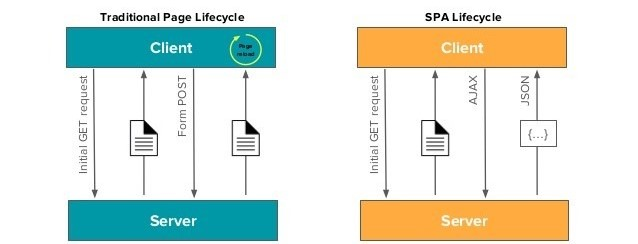
\includegraphics[width=0.61\columnwidth]{images/spa.jpg}
        \end{center}
        \caption{Differenza nel tipo di richieste tra SPA e MPA.}
        \label{fig:spa}
\end{figure}
        
\subsection{Importanza dell'ottimizzazione}
Ad oggi, l'ottimizzazione delle prestazioni è quindi diventata un aspetto cruciale nello sviluppo di applicazioni web. Gli utenti si aspettano interazioni con bassa latenza, caricamenti rapidi e risposte immediate. Questa esigenza mette in risalto l'importanza di bilanciare l'aggiunta di funzionalità sofisticate, con l'offerta di una \emph{User Experience} ottimale.
\\I tempi di caricamento prolungati possono portare a un alto tasso di abbandono delle pagine, riducendo l'opportunità di coinvolgere nuovi utenti. Inoltre, con l'aumentare dell'utilizzo di dispositivi mobili e di conseguenza, di connessioni instabili, l'ottimizzazione diventa ancor più critica per assicurare un'esperienza coerente su diverse piattaforme e condizioni di rete.
Tutto ciò non riguarda solo il lato client, ma coinvolge anche il lato server. Un carico eccessivo sui server può influire negativamente sulla scalabilità, causando ritardi nelle risposte e possibili interruzioni del servizio. L'ottimizzazione deve quindi coinvolgere tutti gli aspetti dell'architettura delle applicazioni web.
\\Nell'implementare ottimizzazioni, sono nati varie soluzioni interessanti. Ad esempio, per gestire task che svolgono molte operazioni di Input/Output si è distinto \textbf{Node.js}, mentre per quanto riguardo l'esecuzione di attività che sfruttano molto la CPU è emerso \textbf{WebAssembly(Wasm)}, in sinergia con l'interfaccia di sistema \textbf{WebAssembly System Interface (WASI)}.

\newpage
\section{Motivazioni e Obiettivi}
\label{sec:Obiettivi}
La crescente complessità delle applicazioni web e l'esigenza di offrire agli utenti esperienze interattive sempre più coinvolgenti hanno portato l'ambito dello sviluppo web a una svolta significativa. Le aspettative degli utenti si sono evolute verso applicazioni che offrano prestazioni reattive, interattività immediata e funzionalità avanzate.
\\È proprio questo insieme di aspettative a essere alla base delle motivazioni che hanno guidato la scelta del tema di questa tesi di laurea.
In particolare, la presente ricerca si propone di esplorare in profondità il complesso equilibrio tra l'implementazione di funzionalità sofisticate (principalmente \textbf{CPU-Intensive}) e l'ottimizzazione delle prestazioni all'interno delle applicazioni web. Il fulcro di questa indagine sarà una comparazione dettagliata tra due approcci di sviluppo distinti per un'applicazione che consenta \textbf{l'elaborazione server-side di immagini} caricate da un utente.
Non verrà esplorato, in modo approfondito il campo dell'elaborazione digitale di immagini, ma ci si limiterà all'implementazione di funzionalità usate spesso da utenti comuni, come ad esempio ridimensionamento, rotazione, aumento/diminuzione di luminosità e contrasto e altre che verranno specificate nel capitolo \ref{chap:3}.
\\Tale tipologia di applicazione, si sposa bene per lo scopo finale della tesi: valutare come due aprrocci (e due linguaggi) piuttosto differenti, ma sempre più diffusi al giorno d'oggi, risolvano il problema di un'applicazione web che svolga operazioni dall'alto costo computazionale.
Le due modalità di sviluppo in questione riguarderanno l'utilizzo delle tecnologie JavaScript e WebAssembly server-side e quindi rispettivamente del runtime environment Node.js e del linguaggio di programmazione Rust in combinazione con WebAssembly System Interface. 
\\Si intende esplorare le opportunità offerte da tecnologie quali WebAssembly e Node.js nell'ottica di un'ottimizzazione delle prestazioni. Questa ricerca mira a comprenderne i benefici specifici, individuando le situazioni in cui uno dei due approcci può risultare più vantaggioso in termini di efficienza computazionale e reattività.
fornendo un'analisi approfondita delle performance e delle prestazioni riscontrate.
\begin{figure}
        \begin{center}
                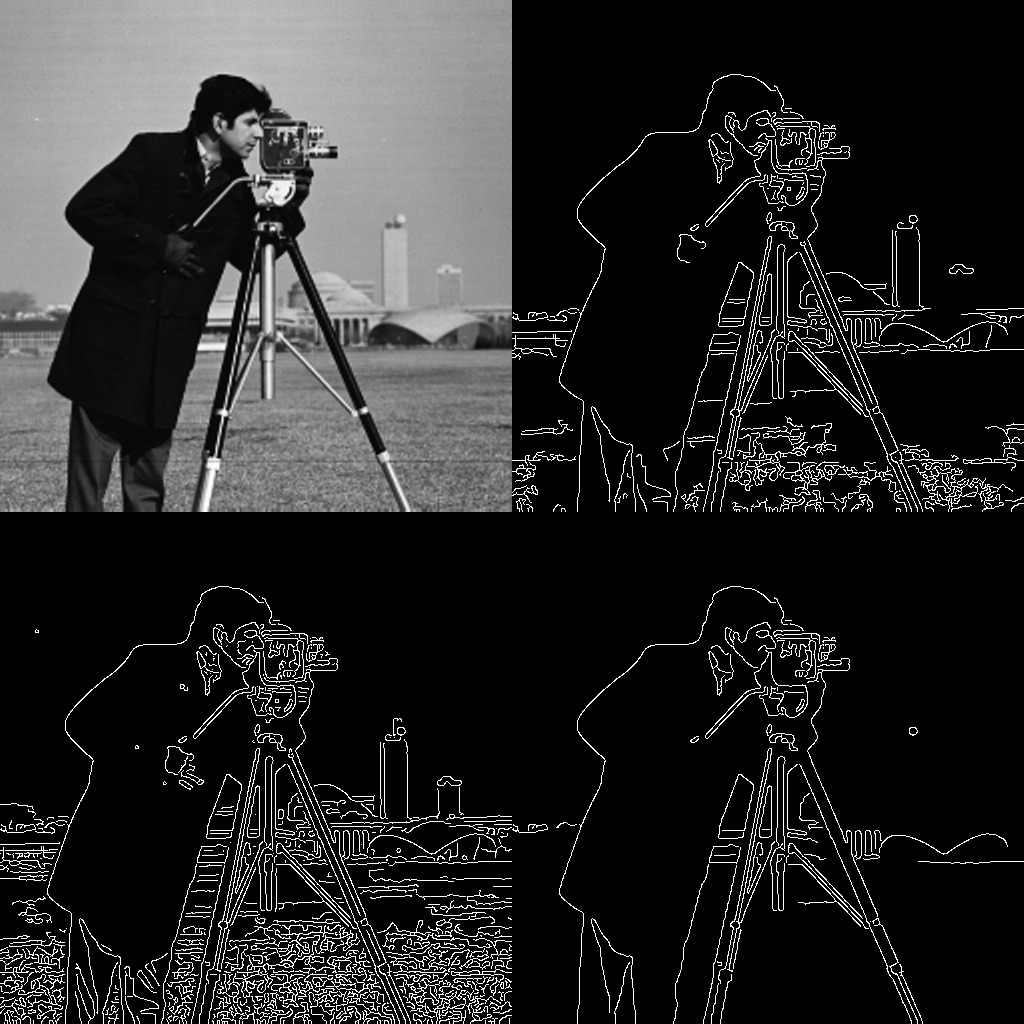
\includegraphics[width=0.6\columnwidth]{images/imageProc.jpg}
        \end{center}
        \caption{Il campo dell'elaborazione digitale di immagini è molto ampio e sarebbe possibile integrare anche operazioni avanzate (edge detection, pattern recognition etc.) che richiederebbero risorse computazionali ancora maggiori, ma per lo scopo di questa tesi ci si limiterà a elaborazioni più semplici.}
        \label{fig:imageProc}
\end{figure}
In particolare, Rust è
\subsection{Analisi Comparativa delle Tecnologie}
Un elemento iniziale di questa ricerca sarà un analisi dettagliata delle tecnologie prese in esame. 
Si partirà con un analisi comparativa delle due tecnologie, presentando i vantaggi e gli svantaggi teorici di entrambe. Sarà infatti fondamentale comprendere come ciascuna affronti la complessità legata ad operazioni I/O-intensive e CPU-intensive per valutare nel modo più opportuno i risultati ottenuti in fase di test e benchmark dell'applicazione sviluppata.
\begin{figure}
        \centering
        \begin{minipage}{0.40\textwidth}
            \centering
            
\includegraphics[width=0.9\textwidth]{images/rustwasm.jpg} % first figure itself
            \caption{Rust e Wasm}
        \end{minipage}\hfill
        \begin{minipage}{0.40\textwidth}
            \centering
            
\includegraphics[width=0.9\textwidth]{images/node.png} % second figure itself
            \caption{Node.js}
        \end{minipage}
    \end{figure}
\subsection{Valutazione dell'Impatto di Wasm}




\section{Trend di evoluzione del web}
\label{sec:Trend}
\subsection{Paradigmi di Sviluppo Moderni}

\subsection{Esperienze Utente Migliorate ?}



\section{Struttura della tesi}
\label{sec:struttura}

This is a reference to a chapter \ref{chap:1}. This is a reference to a figure \ref{fig:doge}. This is a reference to some code \ref{lst:hello}. This is a citation \cite{famous:paper}.

\lstinputlisting[label=lst:hello, firstline=2, lastline=4, caption={I directly included a portion of a file}]{code/hello.py}

\begin{lstlisting}[language=Java, label=lst:java, caption={Some code in another language than the default one}]
public void prepare(AClass foo) {
        AnotherClass bar = new AnotherClass(foo)
}
\end{lstlisting}


\begin{figure}
\begin{center}

\includegraphics[width=0.3\columnwidth]{images/doge.png}
\end{center}
\caption{This is not a figure. It's a caption.}
\label{fig:doge}
\end{figure}

\chapter{Tecnologie utilizzate}
\label{chap:2}

\section{Introduzione alle tecnologie}
\label{sec:IntroduzioneTecnologie}
Come già introdotto brevemente nel capitolo \ref{chap:1}, per lo scopo di questa tesi si è scelto di confrontare due approcci differenti, ma sempre più utilizzati nelle applicazioni web moderne.
In particolare si partirà da WebAssembly e dall'interfaccia di sistema WASI, per finire con un'introduzione anche su Node.js.

\section{WebAssembly}
\label{sec:Wasm}
WebAssembly (Wasm) è uno standard che definisce un formato binario (.wasm) e un relativo formato testuale (.wat) per la scrittura di codice eseguibile nelle pagine web. 
\\Esso è nato come integrazione a JavaScript, per consentire l'esecuzione di codice ad una velocità paragonabile a quella del codice nativo.
\textbf{Il codice WebAssembly è eseguito all'interno di una sandbox garantendo così sicurezza.
I programmi possono essere compilati da svariati linguaggi di alto livello in moduli Wasm. rendendo possibile l'esecuzione di applicazioni lato client in maniera che prima era impensabile.} MODIFICARE!!!
Al giorno d'oggi praticamente ogni browser supporta WebAssembly e il suo sviluppo è portato avanti dal \emph{W3C WebAssembly Working Group}

\subsection{Storia e Origini di WebAssembly}
\subsubsection{I predecessori}
Nel 2011 Google rilasciò un progetto open source chiamato \textbf{Native Client (NaCl)}.
L'obiettivo era quello di consentire l'esecuzione di codice nativo nel browser all'interno di una sandbox con privilegi limitati.
In particolare si stava cercando di supportare software che richiedevano grande sforzo computazionale (simulazioni, elaborazioni di audio e video e giochi).
\\Il progetto si rivelò un successo sotto il punto di vista prestazionale. Vennero infatti rilasciati diversi software e giochi che presentavano prestazioni simili alla rispettiva versione Desktop.
Non mancavano però diversi problemi. Il codice ottenuto era eseguibile solo nel browser Chrome, era impossibile l'interazione con JavaScript o con altre API sul web.
\\Un tentativo di evoluzione fu presentato nel 2013 dal team di Mozilla. Si trattava di \textbf{asm.js}, un sottoinsieme di JavaScript che consentiva l'invocazione di funzioni scritte in linguaggi come C, C++ o Rust, in diversi browser e direttamente da JavaScript.
A discapito di una maggior portabilità ci fu una significativa diminuizione delle prestazioni, dovuta alla lentezza dell'interprete JavaScript.
Queste due soluzioni dimostrarono la possbilità di eseguire codice in una sandbox, o con ottime prestazioni, ma solo all'interno di Chrome (NaCl), oppure in diversi browser ma con prestazioni decisamente inferiori.
Si voleva quindi trovare un modo per unificare gli enormi vantaggi dei due approcci.\cite*{wasmBook}
\subsubsection{L'annuncio}
Fu nel Giugno 2015 che Brendan Eich (creatore di JavaScript), insieme ad altri sviluppatori di Mozilla, annunciarono che lo sviluppo di WebAssembly era cominciato.\cite*{asmjsToWasm}
Wasm venne presentato come "un nuovo standard open source che definiva un formato e un modello di esecuzione portabile, efficiente in termini di dimensioni e tempo di caricamento, specificamente progettato per essere un target di compilazione per il web".
Capendo le potenzialità di ciò che stava venendo sviluppato hanno dato il loro contributo al progetto, aziende del calibro di Google, Microsoft, Apple e Unity.
Nel 2017 venne lanciato il prodotto minimo funzionante (MVP), che conteneva pressochè le stesse funzionalità presenti in asm.js e venne dichiarata conclusa la fase di preview.

\newpage
\subsection{I concetti chiave di WebAssembly}
WebAssembly codifica un linguaggio di programmazione di basso livello, simile ad Assembly. Il linguaggio è strutturato attorno ai seguenti concetti:\cite*{wasmSpec}

\subsubsection{Valori}
In WebAssembly sono presenti 4 tipi di valori numerici. Interi e numeri a virgola mobile, ognuno da 32 o 64 bit (i32, i64, f32, f64), un tipo vector a 128 bit(i128) contenente anch'esso valori numerici (ad esempio da 2 f64, oppure da 4 i32 etc.) ed inoltre è presente un tipo riferimento per puntatori a differenti entità. 
\\Quest'ultimo è definito "opaco", in quanto non è visibile né la loro dimensione, né la loro rappresentazione in bit. Al contrario i primi due tipi sono "trasparenti".
\\Infine è anche possibile la rappresentazione di byte non interpretati grazie al tipo \emph{byte}.
\subsubsection{Istruzioni}
Il modello computazionale di WebAssembly è basato su uno stack. Il codice è costituito da una sequenza di istruzioni eseguite in ordine. Le istruzioni sfruttano un \emph{operand stack} e possono essere di tipo semplice o di controllo.
\\Le operazioni semplici svolgono manipolazioni basilari sui dati, prelevando (\emph{pop}) parametri dallo stack e inserendo il risultato nello stesso (\emph{push}). Le operazioni di controllo, invece alterano il flusso di esecuzione grazie a costrutti condizionali, blocchi e cicli.
\subsubsection{Traps} 
Alcune istruzioni possono fallire e generare degli errori (traps) che non è possibile gestire all'interno di WebAssembly. Tali errori vengono infatti lanciati nell'ambiente di esecuzione dell'host, dove invece vengono normalmente gestiti.
\subsubsection{Funzioni}
Il codice è diviso in funzioni. Ognuna di queste ha una certe sequenza di valori sia come parametri che come tipo di ritorno. In una funzione possono inoltre essere chiamate altre funzioni (anche ricorsivamente) e create variabili locali.
\newpage\subsubsection{Tabelle}
Una tabella è un array di valori "opachi" di un particolare tipo. Tale struttura consente al programma di ottenere i valori indirettamente attraverso un indice dinamico. Tramite le tabelle è possibile, per esempio invocare funzionii indirettamente, emulando così i puntatori a funzione.
\subsubsection{Memoria lineare}
La memoria lineare è un  array continuo di byte. Ha una dimensione iniziale che può crescere dinamicamente al bisogno. Un programma può leggere e scrivere valore in memoria (operazioni di \emph{load/store}), in qualsiasi indirizzo (anche in maniera non allineata).
\subsubsection{Moduli}
Un modulo è l'unità di deployment per un programma WebAssembly. Esso conterrà le definizioni di funzioni, tabelle, memoria etc. In un modulo è anche possibile esportare o importare definizioni, inizializzare tabelle o memoria lineare e anche definire una funzione \emph{start} che verrà eseguita automaticamente. 
\subsubsection{Embedder}
Solitamente un modulo WebAssembly sarà integrato in un host che ne definirà l'inizializzazione, la risoluzione delle funzioni importate  e le modalità di accesso di quelle esportate. L'Embedder è l'entità che implementa la connessione tra l'ambiente host e il modulo Wasm. Ci si aspetta che l'embedder interagisca con la semantica di WebAssembly in un modo ben definito nelle specifiche del formato Wasm.
\begin{figure}
        \begin{center}
                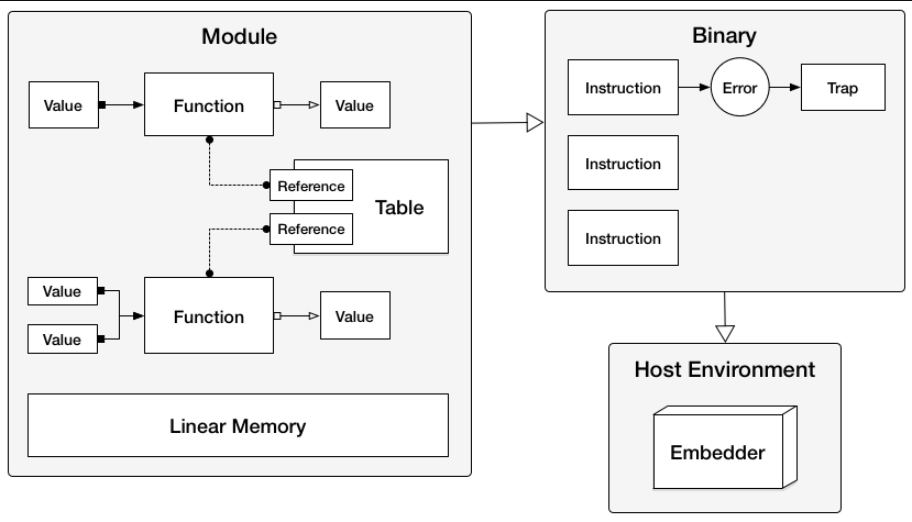
\includegraphics[width=0.9\columnwidth]{images/wasmArchitecture.png}
        \end{center}
        \caption{Architettura di WebAssembly}
        \label{fig:wasmArch}
\end{figure}

\newpage
\subsection{Le fasi semantiche}
Nella semantica di WebAssembly è possibile individuare tre fasi principali: decodifica, validazione ed esecuzione.\cite*{wasmSpec}
\subsubsection{Decodifica}
I moduli WebAssembly sono distribuiti in formato binario (.wasm) e per questo è necessario decodificarli in modo da ottenere una rappresentazione interna del modulo, con cui il web browser o il runtime environment potrà lavorare.
\subsubsection{Validazione}
Dopo aver decodificato i moduli binari, per poterli istanziare, è necessario controllare che questi siano validi.
La validità è verificata grazie ad un sistema di tipi basato sulla sintassi astratta di un modulo e sul suo contenuto. In particolare per ogni componente della sintassi è presente una regola che specifica le condizioni da rispettare perchè il modulo risulti valido.
!!!!Ad esempio viene controllato l'ordine delle istruzioni nel corpo di una funzione assicurandosi che lo stack sia utilizzato nel modo corretto.
Per esempio, dato un contesto \(C\) e un'istruzione del tipo \emph{t.binop} (che rappresenta un'operazione binaria tra tipi numerici, come ad esempio i32.add, f64.xor etc.) è valida con tipo \([t~t]{\rightarrow} [t]\), in notazione formale: 
\begin{equation*}
\frac{
}{
        C {\vdash} t\mathsf{.}{\mathit{binop}} : [t~t] {\rightarrow} [t]
}
\end{equation*}
Oppure con un'istruzione più complicata per l'aumento di memoria lineare \emph{memory.grow}:
\begin{itemize}
        \item La memoria \(C.{\mathit{mems}}[0]\) deve essere definita nel contesto.
        \item Allora l'istruzione risulta valida con tipo \([{\mathit{i32}}] {\rightarrow} [{\mathit{i32}}]\)
\end{itemize}
\begin{equation*}
        \frac{
        C.{\mathit{mems}}[0] = {\mathit{memtype}}
      }{
        C {\vdash} {\mathit{memory.grow}} : [{\mathit{i32}}] {\rightarrow} [{\mathit{i32}}]
      }        
\end{equation*}
\subsubsection{Esecuzione}
Terminata la validazione di ogni istruzione il modulo può finalmente essere istanziato.
L'istanza di un modulo ne è la rappresentazione dinamica. Esso comprende lo stack, sul quale operano le istruzioni WebAssembly e uno \emph{store} astratto, contenente lo stato globale (è la rappresentazione a runtime di tutte le istanze di funzioni, tabelle, memorie etc. che sono state allocate dall'istanziazione).
Terminata l'istanziazione, diventa effettivamente possibile l'esecuzione di istruzioni WebAssembly.
\\In particolare se nel modulo era stata definita una funzione \emph{\_start}, essa sarà eseguita subito dopo la creazione dell'istanza. D'ora in avanti diventerà anche possibile invocare funzioni esportate, chiamandole direttamente dall'istanza.
Per ogni istruzione , è presente una regola che specifica l'effetto della sua esecuzione sullo stato del programma. Rimanendo coerenti con gli esempi sulla validazione, segue il comportamento dell'istruzione \emph{t.binop}:

\begin{itemize}
        \item In seguito alla validazione, possiamo assumere che due valori di tipo \(t\) si trovino in cima allo stack.
        \item Viene eseguita l'operazione di \textbf{pop} del valore \(t.const~c_1\) dallo stack
        \item Viene eseguita l'operazione di \textbf{pop} del valore \(t.const~c_2\) dallo stack
        \item Se \({\mathit{binop}}_t(c_1, c_2)\) è definita allora:
        \begin{itemize}
                \item Sia \(c\) il possibile risultato di \({\mathit{binop}}_t(c_1, c_2)\)
                \item Viene eseguita l'operazione di \textbf{push} del valore \(t.const~c\) nello stack
        \end{itemize}
        \item Altrimenti:
        \begin{itemize}
                \item Trap
        \end{itemize}
\end{itemize}
In notazione formale:
\begin{equation*}
        \begin{split}\begin{array}{lcl@{\qquad}l}
                (t\mathsf{.}{\mathsf{const}}~c_1)~(t\mathsf{.}{\mathsf{const}}~c_2)~t\mathsf{.}{\mathit{binop}} &{\hookrightarrow}& (t\mathsf{.}{\mathsf{const}}~c)
                  & (\mathrel{\mbox{if}} c \in {\mathit{binop}}_t(c_1,c_2)) \\
                (t\mathsf{.}{\mathsf{const}}~c_1)~(t\mathsf{.}{\mathsf{const}}~c_2)~t\mathsf{.}{\mathit{binop}} &{\hookrightarrow}& {\mathsf{trap}}
                  & (\mathrel{\mbox{if}} {\mathit{binop}}_{t}(c_1,c_2) = \{\})
                \end{array}\end{split}
\end{equation*}
\break
Si noti che sia l'istanziazione, che l'invocazione di funzioni, sono operazioni che avvengono all'interno dell'ambiente di esecuzione dell'host.
\begin{figure}
        \begin{center}
                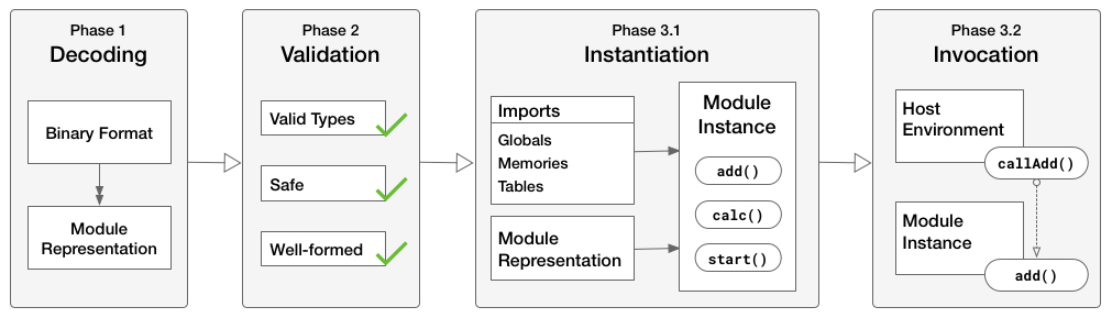
\includegraphics[width=0.97\columnwidth]{images/wasmSemanticPhases.png}
        \end{center}
        \caption{La semantica di WebAssembly}
        \label{fig:wasmPhases}
\end{figure}

\newpage
\subsection{Vantaggi di WebAssembly}
WebAssembly is being created as an open standard inside the W3C WebAssembly Community Group with the following goals:
Be fast, efficient, and portable — WebAssembly code can be executed at near-native speed across different platforms by taking advantage of common hardware capabilities.
Be readable and debuggable — WebAssembly is a low-level assembly language, but it does have a human-readable text format (the specification for which is still being finalized) that allows code to be written, viewed, and debugged by hand.
Keep secure — WebAssembly is specified to be run in a safe, sandboxed execution environment. Like other web code, it will enforce the browser's same-origin and permissions policies.
Don't break the web — WebAssembly is designed so that it plays nicely with other web technologies and maintains backwards compatibility.


\newpage
\section{WebAssembly System Interface}
\label{sec:WASI}
\subsection{Ruolo di WebAssembly System Interface}
\subsection{Rust e WASI}
\subsection{Struttura di WASI}
\subsection{Wasmtime}
\subsection{Applicazioni e Casistiche d'Uso di WASI}

\newpage
\section{Node.js}
\label{sec:Node}
\subsection{Panoramica di Node.js}
\subsection{Vantaggi di Node.js}
\subsection{Ecosistema di Node.js}

\newpage
\section{Confronto tra tecnologie}
\label{sec:Confronto}
\subsection{Prestazioni}
\subsection{Sicurezza}
\subsection{Facilità di Sviluppo}
\subsection{Scalabilità ed Espandibilità}

\newpage
\section{Conclusioni preliminari}
\label{sec:ConclusioniTecnologie}

\newpage
\lstinputlisting[label=lst:hello, firstline=2, lastline=4, caption={I directly included a portion of a file}]{code/hello.py}

\begin{lstlisting}[language=Java, label=lst:java, caption={Some code in another language than the default one}]
public void prepare(AClass foo) {
        AnotherClass bar = new AnotherClass(foo)
}
\end{lstlisting}

\chapter{Prototipo per esecuzione efficiente di codice Wasm con tecniche di Image Processing}
\label{chap:3}
Nel capitolo precedente sono state esaminate le differenze sostanziali tra un'approccio basato su Rust in combinazione con WebAssmebly e uno basato su Node.js.
In questo capitolo si presenterà il prototipo sviluppato con l'obiettivo di comprendere l'impatto di tali differenze in un'applicazione pratica.
\section{Descrizione dell'applicazione}
Il prototipo sviluppato è un applicazione dedicata all'elaborazione digitale di immagini, concepita per simulare un contesto realistico in cui le operazioni richiedono una considerevole quantità di elaborazioni da parte della CPU.
\\Dato il limitato tempo disponibile, non è stato possibile esplorare in dettaglio il vasto campo del \emph{digital image processing}. Pertanto, sono state impiegate librerie preesistenti in entrambi i linguaggi, evitando di immergersi eccessivamente nella programmazione di basso livello.
\\L'architettura dell'applicazione segue un modello client-server in entrambe le implementazioni.
Il cliente ha il compito di fornire i file da elaborare insieme alle relative specifiche sulle modifiche da apportare.
Il server eseguirà le modifiche richieste e restituirà al cliente il percorso della nuova immagine, pronta per il download.
\\Nel processo di selezione delle possibili modifiche da apportare, è stato essenziale individuare due librerie nei rispettivi linguaggi utilizzati.
Successivamente, per garantire uniformità nelle opzioni di modifica disponibili, sono state estratte le seguenti funzionalità comuni: 
\begin{itemize}
    \item ridimensionamento;
    \item rotazione di 90°;
    \item ribaltamento in orizzantale;
    \item conversione in bianco e nero;
    \item regolazione del contrasto;
    \item modifica della luminosità;
\end{itemize}
Tali operazioni sono state selezionate poiché rappresentano funzionalità frequentemente utilizzate anche da utenti comuni, oltre a caratterizzarsi per la loro eterogeneità. Alcune di queste coinvolgono esclusivamente la manipolazione dei pixel, come ad esempio la rotazione e il ribaltamento, mentre altre, come la conversione in scala di grigi o la modifica del contrasto/luminosità, comportano modifiche dirette ai pixel stessi.
\begin{figure}
    \centering
    \begin{minipage}{.5\textwidth}
      \centering
      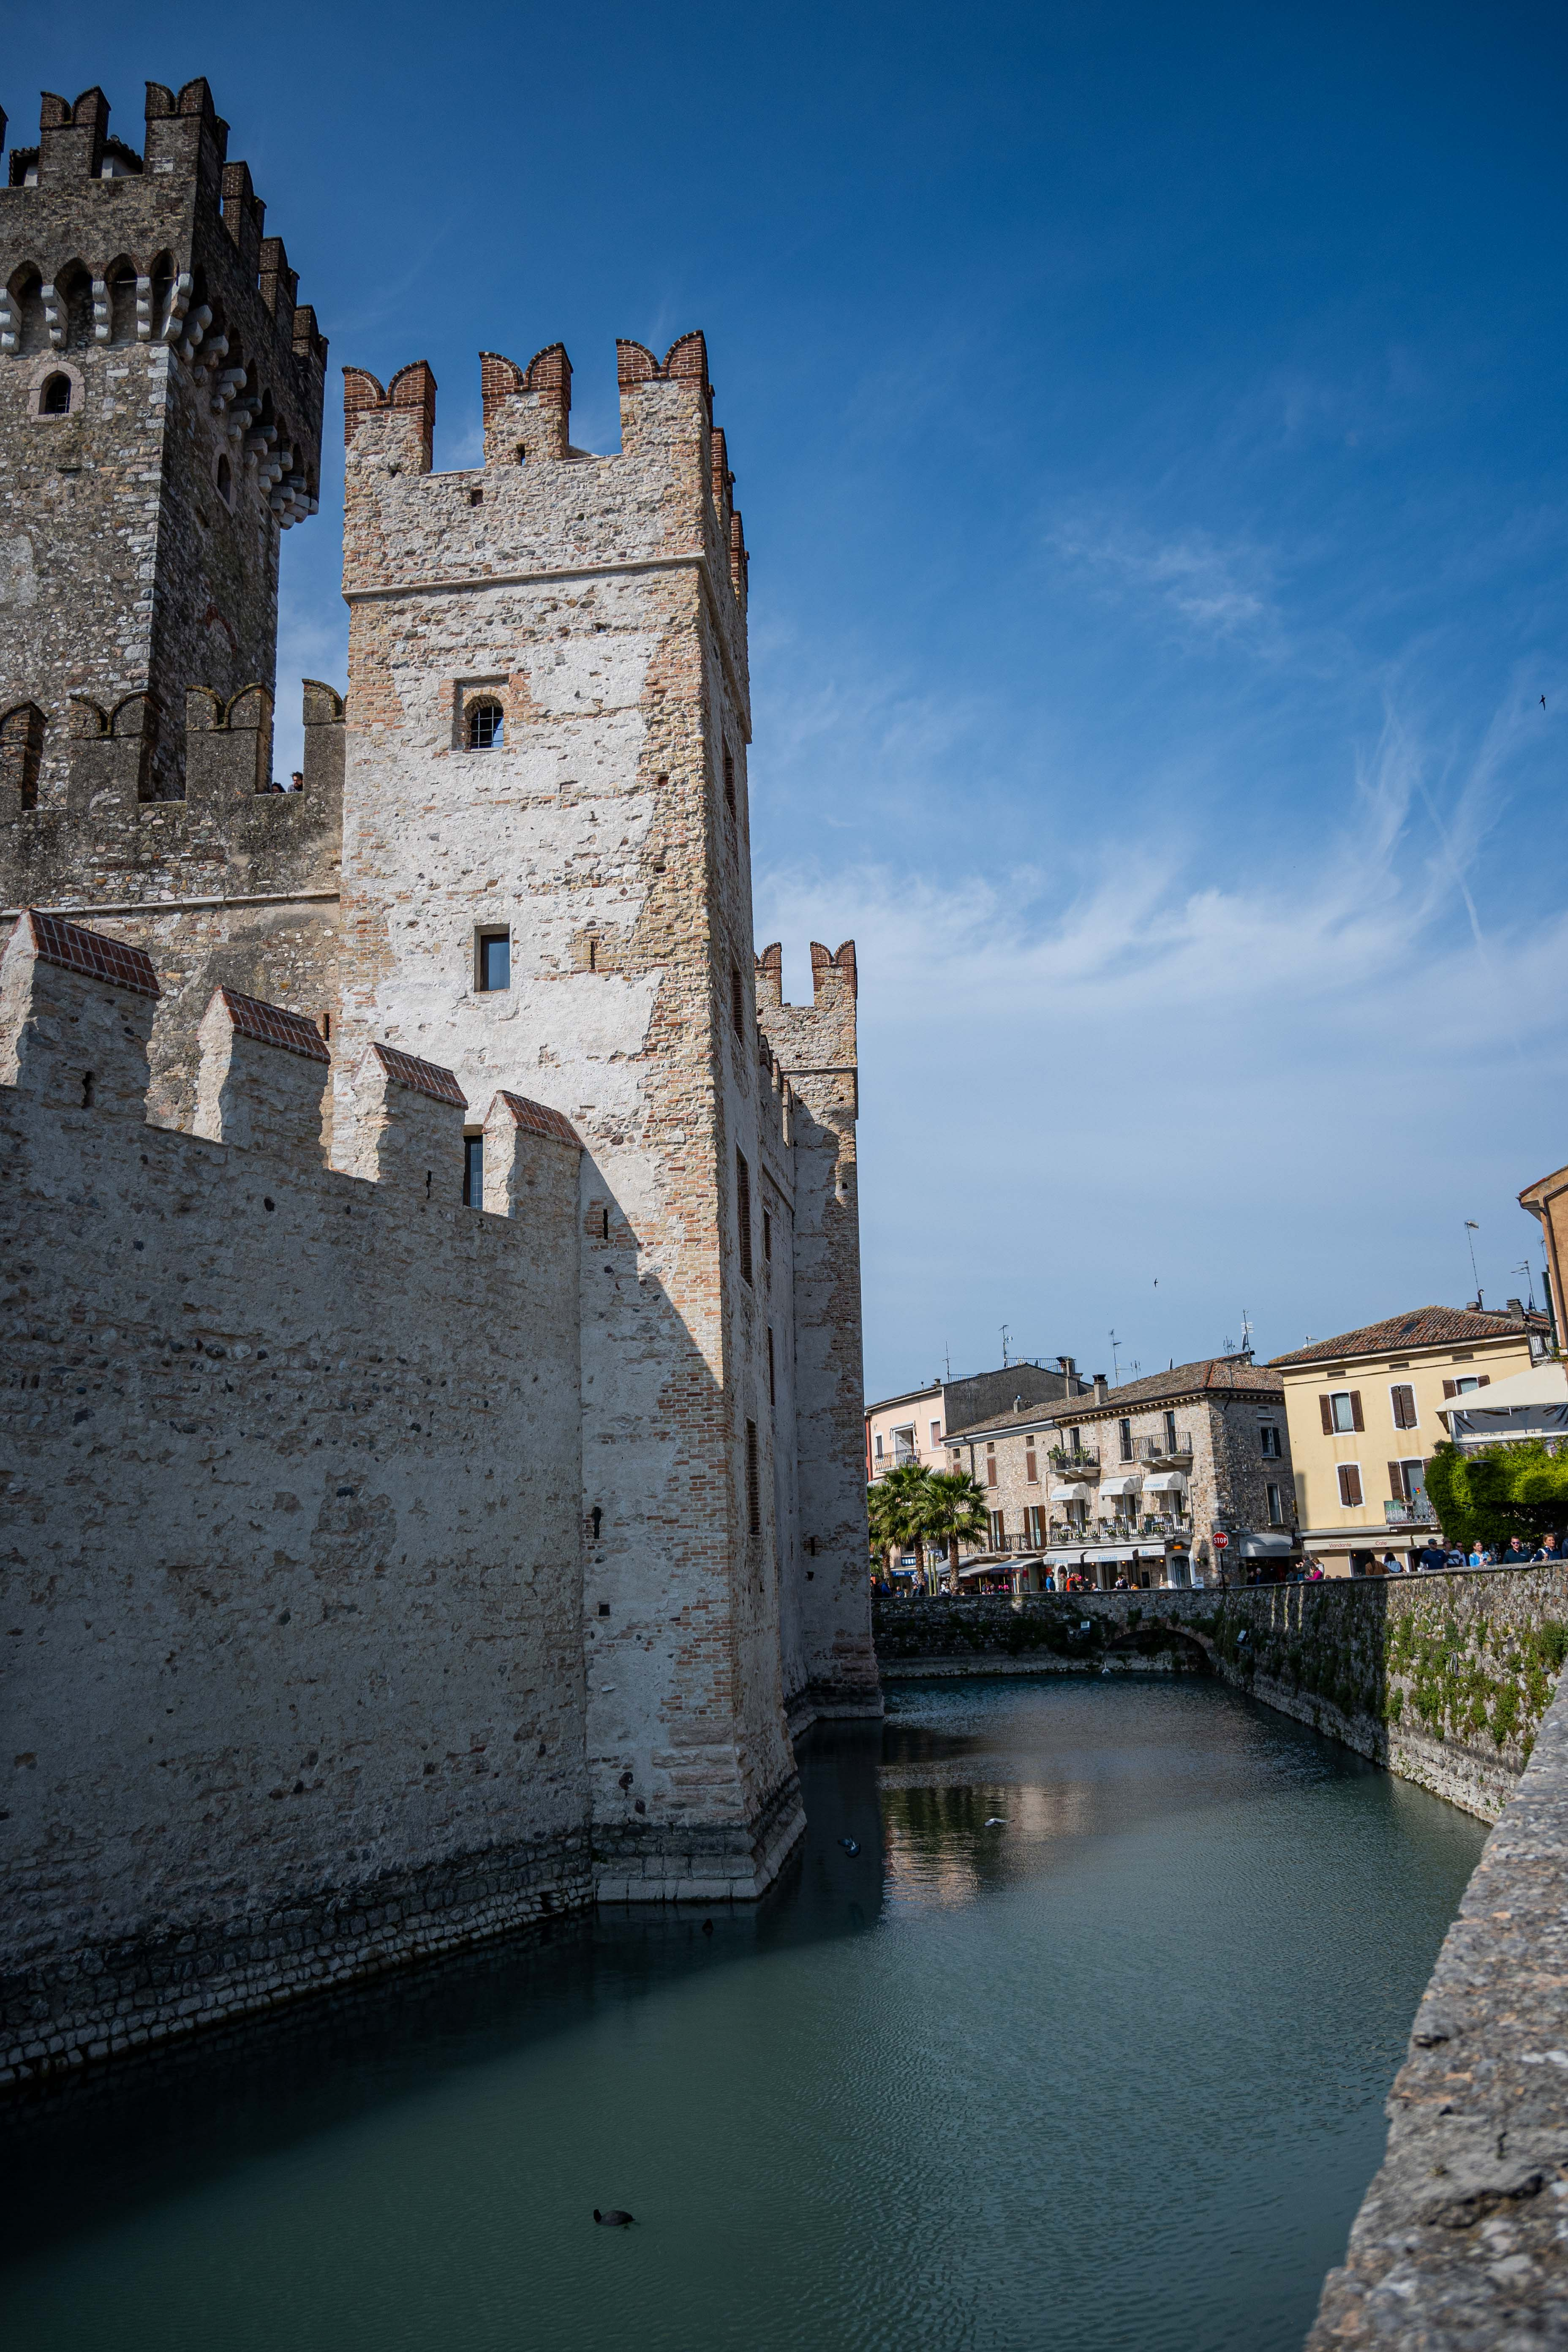
\includegraphics[width=.7\linewidth]{images/pre.jpeg}
    \end{minipage}%
    \begin{minipage}{.5\textwidth}
      \centering
      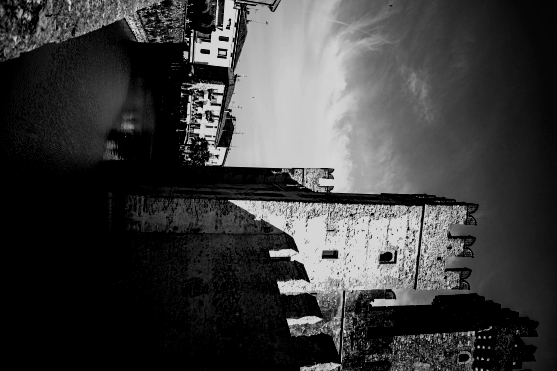
\includegraphics[width=1\linewidth]{images/post.jpg}
    \end{minipage}
    \caption[Esempio immagine pre/post elaborazione]{Esempio di immagine a cui sono state apportate tutte le elaborazioni specificate.}
\end{figure}
\newpage
\section{Implementazione in Rust e Wasm/WASI}
Per quanto riguarda l'implementazione si è deciso di partire dal prototipo sviluppato in Rust poiché rappresentava l'aspetto più innovativo e richiedeva un considerevole impegno in termini di tempo.
\\Si è resa inoltre necessaria la ricerca di un framework che consentisse la creazione di un web server per la gestione delle richieste utente.
\\La scelta è ricaduta su actix-web, un web framework potente ed estremamente veloce per Rust.
\\Il client è costituito una semplice pagina HTML contenente un form per il caricamento delle immagini e due riquadri che mostrano l'immagine pre e post modifiche.
Tale pagina eseguirà una richiesta AJAX al server, inviando il file da elaborare e le relative specifiche sulle modifiche.
\\Terminata l'elaborazione il server restituirà il percorso della nuova immagine pronta per essere scaricata.
\begin{figure}
    \begin{center}
            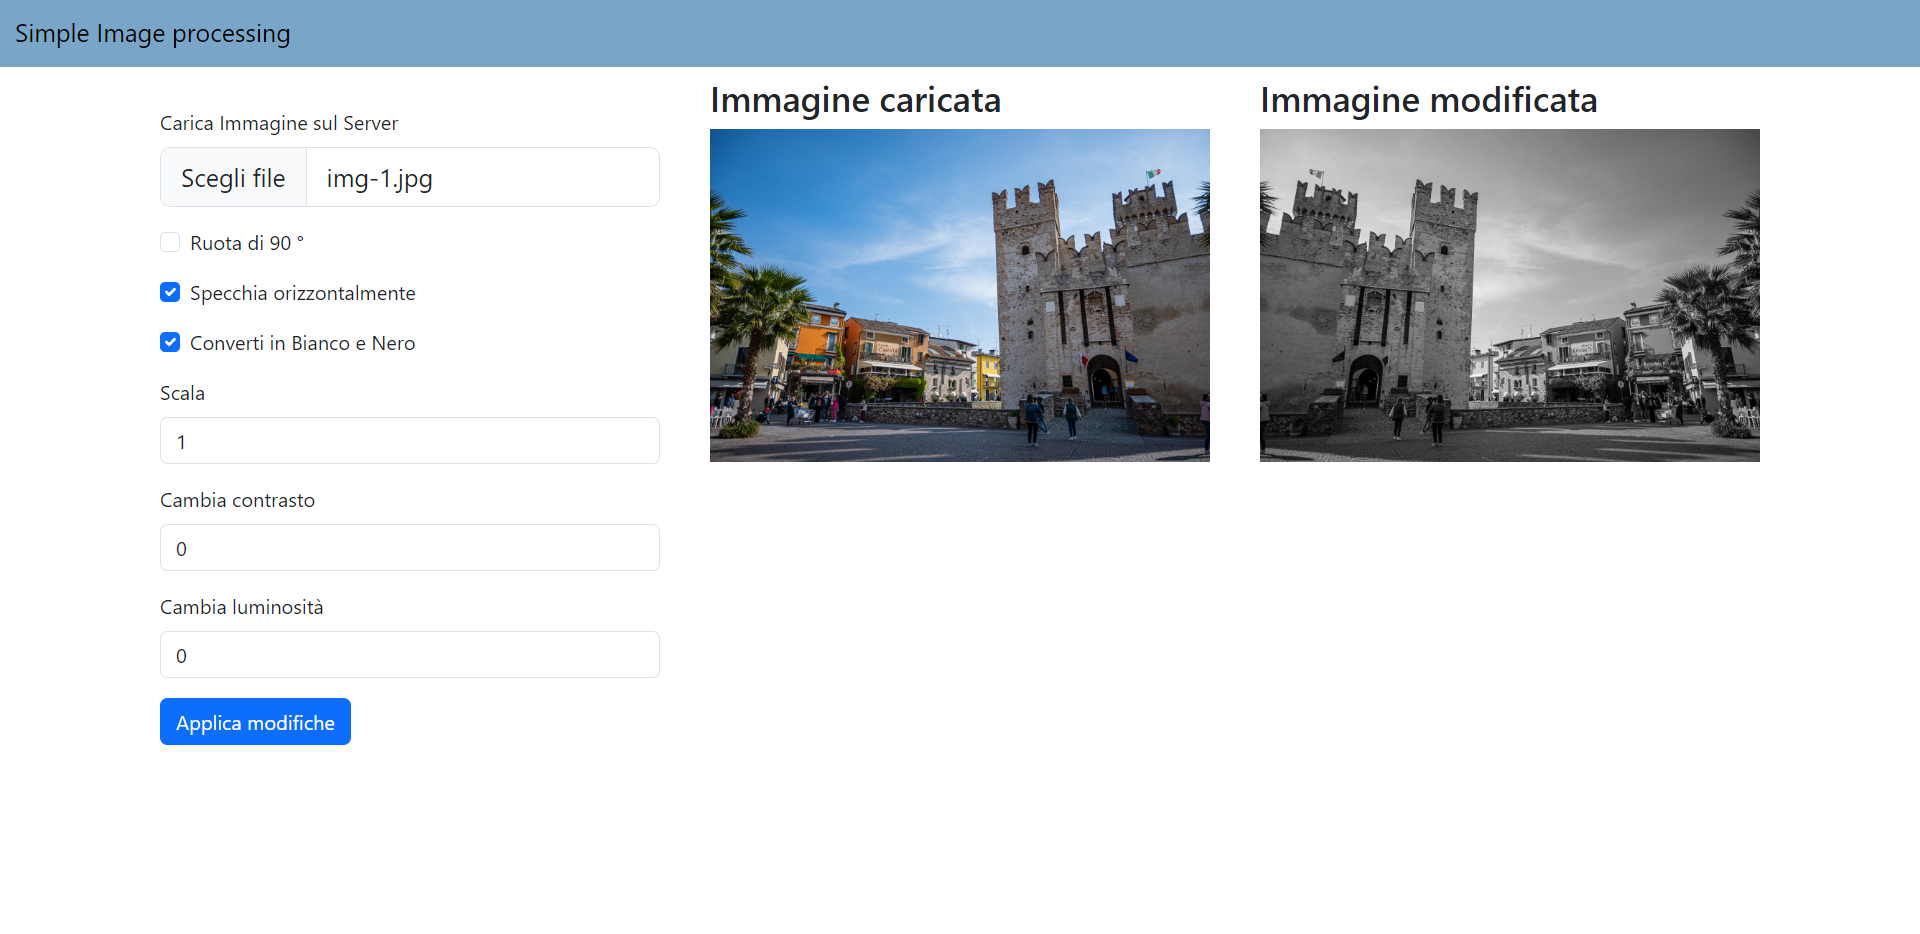
\includegraphics[width=1\columnwidth]{images/client.png}
    \end{center}
    \caption{View nel browser del client}
    \label{fig:client}
\end{figure}
\subsection{Actix-Web}
Lo studio del funzionamento del framework Actix-Web ha costituito un punto focale durante la fase inziale dell'implementazione.
\\Tale framework si è dimostrato estremamente flessibile ed adatto per lo sviluppo del prototipo in questione.
Grazie all'impiego di \textbf{extractors}, di \textbf{handlers} e di altre funzionalità integrate, la gestione di richieste HTTP è risultata intuitiva e diretta.
\\Al fine di garantire un codice più ordinato e manutenibile è stata presa la decisione di strutturare l'applicazione in diversi file.
Tra questi, il file primario è \textbf{main.rs}, che svolge un ruolo centrale nell'architettura complessiva.
\subsubsection{Configurazione server}

\begin{lstlisting}[language=rust, label=lst:RustWasi, caption={Porzione del file main.rs}, showstringspaces=false]
#[actix_rt::main]
async fn main() -> std::io::Result<()> {
    HttpServer::new(move || {
        App::new()
            .route("/", web::get().to(server::handlers::index))
            .route("/upload", web::post().to(server::handlers::upload))
            .service(fs::Files::new("/script", "./src/static/"))
            .service(fs::Files::new("/img", "./img/"))
            .app_data(state.clone())
    })
    .bind("127.0.0.1:8080")?
    .run()
    .await
}
\end{lstlisting}
Nel frammento di codice fornito, viene presentata la creazione di un HttpServer e un'istanza di App tramite il framework Actix-Web.
In Actix-Web, ogni server è costruito attorno a un'istanza di App, che consente di configurare le "regole di routing" per risorse di vario tipo, registrare servizi HTTP e gestire stato di livello applicazione.
\textbf{è presente lo state!!!!! cosa fare???}
\\Nel caso specifico, vengono configurate due regole di routing:
\begin{itemize}
    \item La prima regola gestisce le richieste dirette alla \textbf{home} del sito: in questo caso verrà semplicemente restituita la pagina index.html presente nella directory "static".
    \item La seconda regola gestisce richieste all'endpoint \textbf{upload}, per le quali è necessario ricevere un'immagine e le relative modifiche da apportare all'interno del modulo WebAssembly. Successivamente, verrà restituito il percorso della nuova immagine elaborata.
\end{itemize}
Si sottolinea che entrambe le regole di routing mappano le richieste a funzioni presenti all'interno del file \textbf{handlers.rs} nel modulo server.
\\Successivamente sono stati registrati due servizi HTTP  per garantire l'accesso a risorse statiche: script Javascript e immagini elaborate dall'applicazione.
\\Infine, dopo aver configurato il metodo di dispatching delle richieste ed aver messo a disposizione le risorse necessarie ai client, si è passati alla scrittura del codice nel file \textbf{handlers.rs}. Tale file, come suggerito dal nome, contiene gli handler delle richieste HTTP, con la conseguente esecuzione di codice WebAssmebly per richieste di modifica di immagini.

\begin{lstlisting}[language=Rust,caption={Operazioni principali presenti nel file handlers.rs}, showstringspaces=false]
#[derive(MultipartForm)]
pub struct ImageUpload {
    image: TempFile,
    scala: Text<f32>,
    contrasto: Text<f32>,
    luminosita: Text<i32>,
    ruota: Text<bool>,
    specchia: Text<bool>,
    bw: Text<bool>
}
#[derive(Serialize, Deserialize)]
pub struct Editings{
    scala: f32,
    ...
}
pub async fn index() -> HttpResponse {
    HttpResponse::Ok().content_type("text/html")
        .body(include_str!("../static/index.html"))
}

pub async fn upload(form: MultipartForm<ImageUpload>) -> HttpResponse {
    let time = SystemTime::now().duration_since(SystemTime::UNIX_EPOCH);
    let filepath = format!("img/uploaded/{:?}_{}", time, 
        form.0.file_name.as_str());
    match form.0.image.file.persist(filepath) {
        Ok(_) => {
            let editings = Editings{
                scala : form.0.scala.0,
                ...
            };
            edit(editings)
        },
        Err(e) => {
            HttpResponse::InternalServerError().finish()
        },
    }
}
\end{lstlisting}
Nel codice quì presentato, si possono facilmente notare i due endpoint del prototipo: la funzione \textbf{index()} per richieste alla pagina home e la funzione \textbf{upload()} per richieste di elaborazione di immagini.
\\Per quanto riguarda la prima tipologia si risponde ai client semplicemente fornendo il file HTML statico "index.html".
\\Al contrario la gestione delle richieste di upload è notevolmente più articolata e per questo motivo coinvolge una funzione di supporto denominata \textbf{edit()}. Sarà questa funzione che si occuperà dell'istanziazione del modulo WebAssmebly/WASI e della sua esecuzione.
\\Si sottolinea anche il parametro ricevuto dalla funzione "upload": un \textbf{MultipartForm<ImageUpload>}.
Il framework Actix-Web, con il supporto del crate actix-multipart semplifica notevolmente la gestione di richieste provenienti da form html, anche in presenza di campi di input di tipo "file".
\\Ogni campo definito nella struttura "ImageUpload" corrisponde a un parametro proveniente dalla richiesta HTML e viene automaticamente popolato prima dell'invocazione dell'handler, consentendo un accesso immediato ai valori inviati al server.
\\In sintesi la funzione \textbf{upload()} rende persistente il file temporaneo ricevuto ed inoltre crea un ulteriore \emph{struct} di supporto (\textbf{Editings}) che verrà sfruttata dalla funzione \textbf{edit()} per velocizzare il successivo accesso alle elaborazioni da effettuare.
\\Va sottolineato che "edit()" viene invocata solo se il file è stato reso persistente senza errori. Infatti, tale funzione si occupa dell'istanziazione del modulo WebAssembly e non ha senso tentare di eseguire modifiche su un file che non è stato salvato correttamente.
\subsection{Integrazione modulo Wasm/WASI}
Come precedentemente indicato, per l'esecuzione di codice WebAssmebly, si è deciso di utilizzare il runtime environment \textbf{Wasmtime}.
La sua integrazione all'interno di un'applicazione Rust è resa possibile primariamente grazie ai crate \textbf{wasmtime}, \textbf{wasmtime-wasi} e \textbf{wasi-common}.
\subsubsection{Scambio di dati}
Prima ancora di iniziare l'implementazione è stato fondamentale trovare un modo per \textbf{scambiare dati} tra il modulo WebAssmebly e l'host.
\\Per soddisfare i requesti imposti in questa tesi, è necessario che il modulo WebAssmebly riceva tutte le elaborazioni da effettuare su un'immagine e il nome del file da modificare, ma come introdotto in sezione \ref{subsub:Valori}, una funzione WebAssmebly può ricevere solamente valori di \textbf{tipo numerico}.
\\Analizzando le API WebAssmebly e WASI sono emerse diverse soluzioni a questo problema. Tra queste l'utilizzo della memoria lineare, la scrittura su file, la modifica di variabili d'ambiente o la comunicazione attraverso standard input.
Tuttavia, alcuni di questi approcci potrebbero risultare complessi da implementare e considerando che per l'applicazione sviluppata sarebbe stato sufficiente scambiare una stringa per ottenere tutte le informazioni necessarie, si è scelto di adottare la comunicazione tramite \textbf{standard input}.
\\Nello specifico, per consentire lo scambio di dati tra host e guest, verrà implementato un protocollo composto dalla seguente sequenza di operazioni:
\begin{itemize}
    \item Serializzazione in formato JSON della struct "Editing" contenente tutte le elaborazioni  e il nome del file da modificare;
    \item Inserimento sullo standard input del modulo Wasm, della stringa ottenuta dalla serializzazione;
    \item Lettura della stringa da standard input all'interno del modulo, sfruttando le API messe a disposizione da WebAssmebly System Interface;
    \item Deserializzazione in una Struct Editing equivalente a quella di partenza;
\end{itemize}
Si noti che, se necessario, questo protocollo potrebbe essere applicato anche per ottenere strutture dati in output dal modulo WebAssembly.
\subsubsection{Condizioni necessarie per l'esecuzione}
Prima di poter eseguire un modulo tramite Wasmtime, sono necessarie diverse operazioni preliminari.
\\Dopo aver serializzato la struttura dati e predisposto una \textbf{ReadPipe} (crate wasi-common) per mettere a disposizione la stringa serializzata su standard input, la prima operazione necessaria è la creazione dell'\textbf{Engine} Wasmtime.
\\Esso rappresenta un contesto globale per la compilazione e l'esecuzione di moduli Wasm, che nel nostro specifico caso adotterà la configurazione di default.
\\Si procederà poi con l'istanziazione di un \textbf{wasmtime::Linker}. Il linker faciliterà l'istanziazione del modulo Wasm, risolvendo le diverse import (tra cui quelle per le syscall WASI).
\\Non bisogna poi dimenticare, che a causa dell'architettura di WASI, sarà possibile accedere ed utilizzare i file presenti in una certa directory, solamente se al programma sono state fornite le \textbf{capabilities} necessarie. 
\\Per ottenere le capabilities per operare sulle immagini caricate dagli utenti, è necessario aprire la cartella "img" prima dell'istanziazione del modulo WASI.

\begin{lstlisting}[language=rust, caption={File handlers.rs: operazioni preliminari}, showstringspaces=false]
pub fn edit(editing : Editings) -> HttpResponse {
    let serialized_input = serde_json::to_string(&editing);
    let stdin = ReadPipe::from(serialized_input);
    
    let engine = Engine::default();
    
    let mut linker: Linker<WasiCtx> = Linker::new(&engine);
    wasmtime_wasi::add_to_linker(&mut linker, |s| s); 
    let  image_directory = Dir::open_ambient_dir("img", ambient_authority());
    ...
}
\end{lstlisting}
A questo punto è possibile creare e configurare un contesto WASI tramite la struct \textbf{wasmtime\_wasi::WasiCtxBuilder}.
\\Tramite tale oggetto si specifica che lo standard input sarà prelevato dall'oggetto contenente la serializzazione, lo standard output e lo standard error saranno ereditati dalla macchina host ed infine si fornisce una directory precedentemente aperta, che sarà disponibile al percorso "img".
\\Sfruttando il contesto WASI è ora possibile la creazione dello \textbf{Store} Wasmtime, l'oggetto designato per l'effettiva istanziazione del modulo WebAssembly e che successivamente conterrà tutte le funzioni, la memoria, le tabelle e lo stato interno del programma.
\begin{lstlisting}[language=rust,caption={File handlers.rs: creazione di contesto WASI e Store}, showstringspaces=false]
    let builder = WasiCtxBuilder::new()
    .stdin(Box::new(stdin.clone()))
    .inherit_stdout()
    .inherit_stderr()
    .preopened_dir(image_directory,"img");
    let wasi = builder.build();
    
    let mut store = Store::new(&engine, wasi);
\end{lstlisting}
Ora risulta possibile la creazione del \textbf{Module} WebAssmebly e il suo collegamento con il Linker per poi ottenere, tramite quest'ultimo, un'\textbf{istanza} relativa al Module e allo Store specificati nel metodo \emph{linker.instantiate()}.
\newpage
\begin{lstlisting}[language=rust,caption={File handlers.rs: istanziazione modulo Wasm}, showstringspaces=false]
    let module = Module::from_file(&engine, "src/server/image_proc_module.wasm");
    linker.module(&mut store, "", &module) 
    let instance = linker.instantiate(&mut store, &module);
\end{lstlisting}
\subsubsection{Esecuzione del modulo WebAssmebly}
Avendo configurato Store e contesto WASI, il programma possiede già tutti gli argomenti necessari per il corretto funzionamento e l'unico passo rimanente consiste nell'effettiva esecuzione della funzione del modulo WebAssmebly.
\\Per fare ciò è  necessario ottenere un'istanza di \textbf{wasmtime::Func} tramite l'operazione \emph{get\_typed\_func()} sull'istanza WebAssmebly.
A questo punto l'invocazione della funzione richiesta è finalmente possibile grazie al metodo \emph{Func::call()}.
\\Ad esecuzione terminata verrà eliminato lo store dalla memoria e restituito il percorso dell'immagine modificata al cliente.
\begin{lstlisting}[language=rust,caption={File handlers.rs: invocazione funzione \_start presente nel modulo Wasm}, showstringspaces=false]
    let instance_main = instance.get_typed_func::<(), ()>(&mut store, "_start");
    instance_main.call(&mut store, ());
    drop(store);
    HttpResponse::Ok()
    .content_type("text/plain")
    .body(e.modified_file_path)
\end{lstlisting}
Si noti che in questi esempi di codice non è presente alcuna gestione degli errori. Tuttavia nel prototipo sviluppato, l'utente finale otterrà il nuovo percorso del file, solo nel caso in cui ciascuna delle operazioni illustrate sarà andata a buon fine.
\newpage
\subsection{Modulo WebAssmebly/WASI}
Il modulo WebAssmebly risulta a questo punto piuttosto semplice.
\\Esso si occupa infatti della lettura dei parametri da \textbf{standard input} e della loro deserializzazione in una struct Editings.
\\Successivamente vengono utilizzati i metodi forniti dal crate \textbf{image} di Rust per aprire l'immagine ricevuta, modificarla secondo le specifiche dell'utente e salvarla nel percorso specificato.\cite{rust:image}

\begin{lstlisting}[language=rust, caption={Codice Rust che successivamente verrà compilato in WebAssembly}, showstringspaces=false]
#[derive(Serialize, Deserialize)]
pub struct Editings{
    scala: f32,
    ...
}
fn main() {
    let mut serialized_params = String::new();
    std::io::stdin().read_to_string(&mut serialized_params);
    let editings : Editings = serde_json::from_str(&serialized_params);
    let mut img = image::open(editings.filepath)
    if editings.scala != 0.0 {
        let new_width = (img.width() as f32) * editings.scala;
        let new_heigth = (img.height() as f32) * editings.scala;
        img = img.resize(new_width as u32, new_heigth as u32, image::imageops::FilterType::Nearest);
    }
    if editings.ruota {
        img = img.rotate90();
    }
    ...
    img.save(editings.modified_filepath);
}
\end{lstlisting}
Terminata l'esecuzione del modulo, il controllo ritornerà all'host che si occuperà dell'invio di una risposta adeguata al client:
\begin{itemize}
    \item Se durante l'esecuzione del modulo Wasm tutte le operazioni sono terminate correttamente verrà restituito il percorso della nuova immagine generata;
    \item Altrimenti verrà restituito un messaggio di errore;
\end{itemize}
Terminata la scrittura del codice, è necessaria la compilazione per ottenere un modulo WebAssmebly utilizzabile da wasmtime.
\\Ciò si può fare agovelmente grazie al package manager \textbf{cargo}, ed in particolare grazie al seguente comando:
\begin{lstlisting}[language=Bash, numbers=none]
cargo build --release --target wasm32-wasi
        Compiling image_proc_module v0.1.0 (.\image_proc_module)
            Finished release [optimized] target(s) in 1.21s
\end{lstlisting}
In questo caso risulta pressochè obbligatoria la presenza del flag \textbf{- - release}, in quanto diverse funzioni del crate image, sono estremamente lente se utilizzate in debug mode.
\\Infine si sottolinea che avendo svolto tutte le operazioni necessarie nel main, nel momento in cui l'host invocherà il metodo \emph{get\_typed\_func()}, sarà necessario specificare la funzione denominata \textbf{\_start}.



\newpage
\section{Implementazione in Node.js}
Dopo aver terminato l'implementazione del prototipo mediante l'utilizzo di Rust e WebAssmebly, si è proceduto con l'implementazione di un applicazione dotata delle medesime funzionalità, questa volta utilizzando il runtime environment \textbf{Node.js}.
\\La seconda implementazione è risultata notevolmente più immediata.
In particolare è stato possibile riutilizzare il client sviluppato precedentemente, senza necessità di un'analisi approfondita per l'integrazione di un modulo WebAssmebly.
Come verrà sottolineato in seguito, ciò ha permesso di ottenere un \textbf{codice} decisamente più \textbf{pulito} e di lunghezza proporzionata alla semplicità dell'applicazione sviluppata.
\\La ricerca si è dunque focalizzata sulla selezione di un moduli adeguati per la creazione di un'applicazione web in grado di supportare l'upload e l'elaborazione di immagini.
La scelta è ricaduta sul web framework \textbf{express.js}, in combinazione con il middleware \textbf{multer} e la libreria \textbf{Jimp}.
\subsection{Express.js}
Express.js è un \textbf{web framework} che semplifica lo sviluppo di applicazioni web robuste e scalabili. Esso è stato riconosciuto come lo \textbf{standard de facto} in quest'ambito.
\\Il design di Express è relativamente minimale, tuttavia, grazie all'impiego di \textbf{plugin} e \textbf{middleware} come Multer, è in grado di fornire una vasta gamma di funzionalità.
\\Il framework inoltre rende più semplice il routing, gestendo richieste e risposte HTTP in modo semplice e diretto.
\\Per quanto concerne la nostra applicazione, dopo aver importato i moduli richiesti, è essenziale effettuare una configurazione breve ma precisa, per la gestione delle richieste necessarie e per la configurazione dell'upload dei file.
\begin{lstlisting}[language=JavaScript, caption={Configurazione Express.js}, showstringspaces=false]
    const express = require('express');
    const app = express()
    const port = 3000
        
    app.use(express.static('./static'))
    app.use(express.static('./img/modified'))
    
    app.post('/upload', upload.single('image'), (req, res) => {
      try{
      ...
      }
      } catch (error){
        console.log(error);
        res.status(500).send('Error processing the file');
      }
    })
    
    app.listen(port, () => {
      console.log(`Server listening on port ${port}`)
    })
\end{lstlisting}
Nello specifico viene creata un'applicazione Express tramite l'omonimo metodo \emph{express()}.
\\Successivamente tramite i metodi \emph{express.use(express.static(...))} vengono rese accessibili ai client le directory "static"(contenente il file HTML della home e gli script correlati) e "img/modified" (necessaria per il download delle immagini elaborate dal server).
\\Il server viene poi messo in ascolto sulla porta 3000 e configurato per gestire richieste di tipo POST dirette all'endpoint "/upload".
\\A questo punto, per la corretta gestione del caricamento di immagini, risulta necessario configurare l'applicazione affinché sia in grado di ricevere richieste con Content-Type "multipart/form-data".
\subsection{Multer}
Come introdotto inizialmente, per la gestione di richieste provenienti da un form contenente campi di input di tipo file, è stato adottato il middleware \textbf{multer}.
\begin{lstlisting}[language=Javascript, caption={Configurazione upload immagine}, showstringspaces=false]
const multer  = require('multer');
const storage = multer.diskStorage({
    destination: 'img/uploaded/',
    filename: (req, file, cb) => {
    cb(null, file.originalname);
    }
});
const upload = multer({ storage });
app.post('/upload', upload.single('image'), (req, res) => {
    ...
})
\end{lstlisting}
Una volta importato questo modulo, è necessario impostare, tramite il metodo \emph{multer.diskStorage()}, la destinazione (per coerenza viene mantenuta la directory img/uploaded) e il nome del file appena caricato (viene utilizzato lo stesso nome del file fornito dall'utente).
\\In seguito attraveso l'utilizzo del metodo \emph{multer()} otteniamo un'istanza, tramite la quale è possibile specificare, nei parametri della callback function per richieste all'endpoint upload, che un singolo file dovrà essere reso persistente, come precedentemente specificato nella variabile storage.
\subsection{Jimp}
Una volta terminata la configurazione del server tramite express.js, è possibile procedere con la modifica del file ricevuto. 
\begin{lstlisting}[language=Javascript,caption={Elaborazione immagine grazie ai metodi della libreria Jimp}, showstringspaces=false]
app.post('/upload', upload.single('image'), (req, res) => {
  try{
    const uploadededFilePath =                               'img/uploaded/' + req.file.originalname
    const newFileName =  Date.now() + req.file.originalname 
    const modifiedFilePath = 'img/modified/' + newFileName;

    Jimp.read(uploadededFilePath, (err, img) => {
      if (err) throw err
      else{
        img.scale(req.body.scala)
           .rotate(req.body.ruota)
           .mirror(req.body.specchia,false)
           .contrast(req.body.contrasto/100)
           .brightness(req.body.luminosita/100, function(){
              if(req.body.bw) img.grayscale()
              img.write(modifiedFilePath, function(){
                res.status(200).send(newFileName);
              });
          });
      }
    });

  } catch (error){
    res.status(500).send('Error processing the file');
  }
}
\end{lstlisting}
Il file è aperto mediante l'impego del metodo \textbf{Jimp.read()}, il quale fornisce un'istanza utilizzabile per moodificare l'immagine secondo specifiche.
Quest'ultime si possono essere acquisite  tramite l'oggetto req.body, passato alla callback function \emph{app.post('/upload',...)}.
\\Dopo aver apportato le opportune modifiche all'immagine, essa viene salvata nella cartella "img/modified" con un nuovo nome al fine di garantire univocità tra i vari file.
\\Infine, se tutte le operazioni precedenti vengono eseguite correttamente, verrà restituito all'utente il percorso dell'immagine modificata. In caso contrario, verrà restituito un messaggio di errore.
\newpage
\section{Metodologia di test}
Per valutare le performance di ciascuna implementazione presentata, si è deciso di eseguire lo stesso \textbf{set di test} su entrambe.
\\In particolare è stata scelta un'elaborazione specifica tra quelle disponibili e durante la sua esecuzione sono stati misurati diversi parametri.
\\Per scegliere la tipologia di operazione si è empiricamente tentato di capire quale fosse, tra le elaborazioni implementate, quella più computazionalmente complessa.
Eseguendo vari test su una stessa immagine e verificando la latenza è stato scelto il \textbf{resize} di un'immagine ed in particolare il resize del 10\% (x0.9), , al fine di manipolare un elevato numero di pixel e ottenere un'immagine di dimensioni simili a quella iniziale.
\\In seguito sono state scelte le immagini di test e i parametri da misurare.
Per quanto riguarda le immagini, si è scelto di utilizzare tre file con dimensione crescente:
\begin{itemize}
    \item 1114 x 742 (0.82 Megapixel, 925 KiloByte);
    \item 2869 x 1912 (5.48 Megapixel, 4.63 MegaByte);
    \item 5578 x 3712 (20.7 Megapixel, 17.4 MegaByte);
\end{itemize}
Come parametri da misurare si è deciso di focalizzarsi su:
\begin{itemize}
    \item Latenza per ogni richiesta;
    \item Utilizzo di CPU;
    \item Consumo di memoria;
\end{itemize}
\section{Setup sperimentale}
Per eseguire i test presentati è stato utilizzato un laptop con processore Intel Core i5-10210 (1.6 - 2.10 GHz), 8 GigaByte di Ram e sistema operativo Windows 11.
Per quanto riguarda i software utilizzati, si sono scelte le ultime versioni al momento disponibili:
\begin{itemize}
    \item Rust 1.71
    \item Wasmtime 11.0
    \item Node 18.17.1 (LTS)
\end{itemize}
Il seguente setup, pur non essendo propriamente tipico di un server, ha comunque permesso di osservare differenze notevoli tra i due apprrocci esaminati.
\section{Valutazione delle prestazioni}
Per ottenere un campione di risultati affidabile sono state eseguite 10 misurazioni per ogni immagine.
In seguito sono stato calcolati il valore medio del campione, ottenuto come media aritmetica e la deviazione standard:
\begin{equation*}
    E[X]=\frac{1}{n}\sum_{i=0}^{n}x_i
\end{equation*}
\begin{equation*}
    \sigma_X = \sqrt{\frac{1}{n}\sum_{i=0}^{n}(x_i-E[x])^2}
\end{equation*}
Successivamente verranno presentati i grafici per ciascuno dei parametri scelti, utilizzando rispettivamente Rust in combinazione con WebAssembly e Node.js. Ogni grafico conterrà i risultati per ognuna delle tre immagini utilizzati, consentendo così anche una facile analisi visiva.
\subsection{Latenza}
Il primo parametro misurato è stato quello della latenza.
\\Nello specifico si è analizzato il tempo intercorso tra l'invio di una richiesta di elaborazione e la successiva risposta contenente il percorso della nuova immagine elaborata.
\\Per quanto riguarda Rust si sono ottenuti i seguenti risultati sperimentali:
\begin{align*}
    E[X]_{small}&=850ms,  & \sigma_X=154.94ms\\
    E[X]_{medium}&=1487ms, & \sigma_X=144.99ms\\
    E[X]_{large}&=4212ms,  & \sigma_X=169.95ms
\end{align*}
Relativemente a Node.js invece:
\begin{align*}
    E[X]_{small}&=704ms,  & \sigma_X=79.19ms\\
    E[X]_{medium}&=3081ms, & \sigma_X=240.58ms\\
    E[X]_{large}&=11335ms,  & \sigma_X=282.73ms
\end{align*}
\begin{figure}
    \begin{center}
            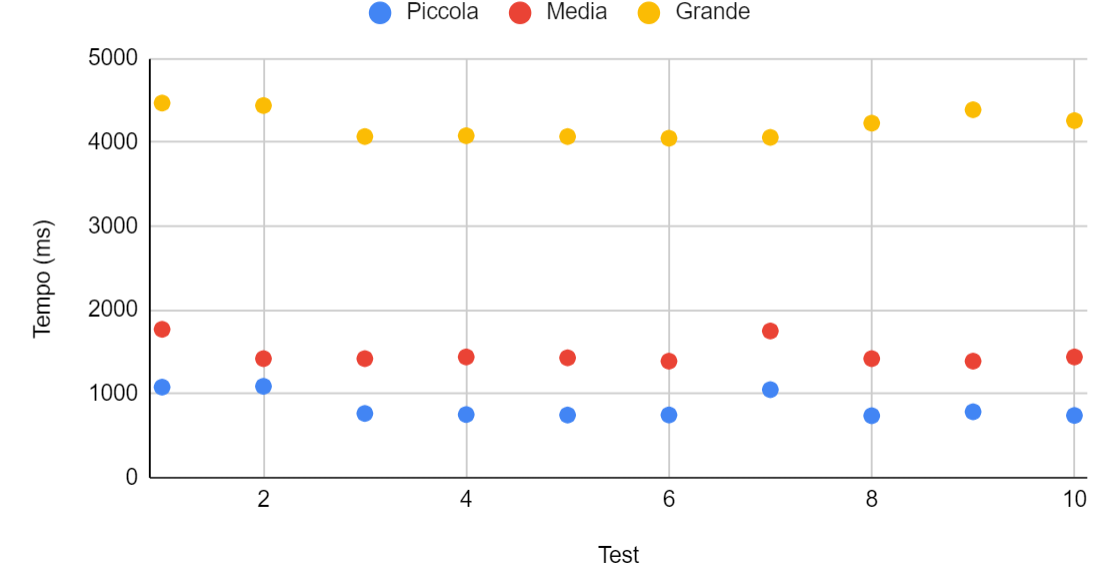
\includegraphics[width=1\columnwidth]{images/rust_latenza.png}
    \end{center}
    \caption{Latenza misurata utilizzando Rust in combinazione con WebAssembly.}
\end{figure}
\begin{figure}
    \begin{center}
            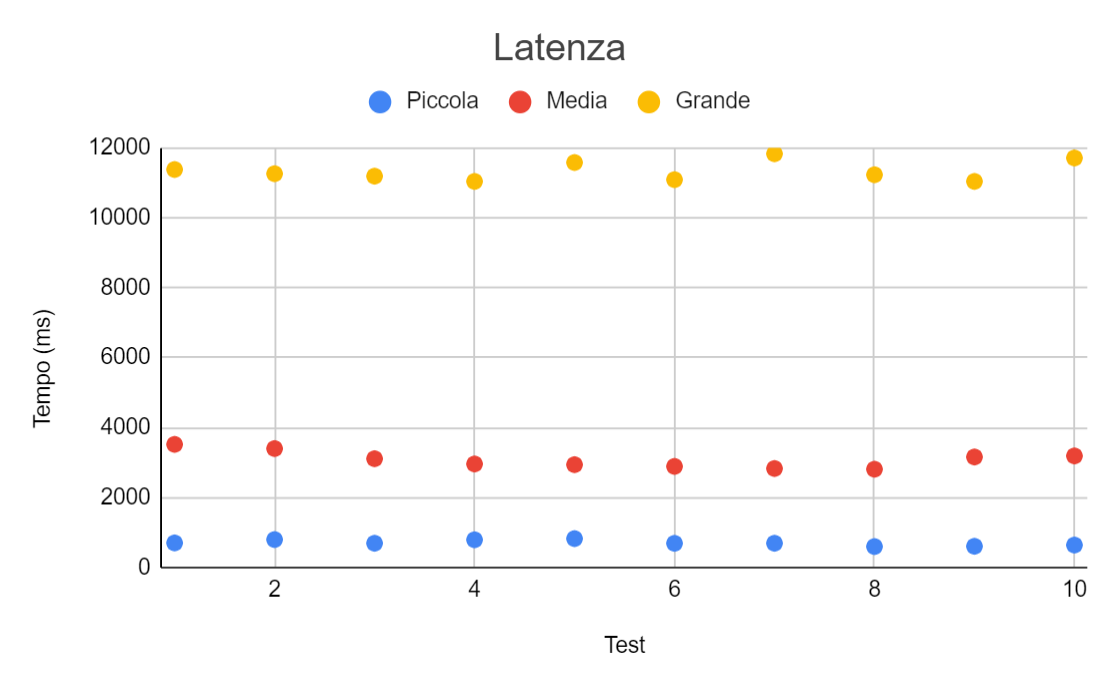
\includegraphics[width=1\columnwidth]{images/node_latenza.png}
    \end{center}
    \caption{Latenza misurata utilizzando Node.js}
\end{figure}Come si può notare il tempo di latenza risulta confrontabile solamente durante l'elaborazione dell'immagine con dimensione minore. Durante l'elaborazione delle rimanenti due immagini, WebAssembly ha ottenuto performance notevolmente migliori, richiedendo circa un terzo del tempo necessario a Node.js per l'elaborazione dell'immagine più grande.
\\È plausibile ipotizzare che, durante la modifica di immagini di piccole dimensioni, WebAssembly non riesca a mettere in evidenza i suoi vantaggi, soprattutto a causa dell'overhead introdotto dalla creazione di un'istanza del modulo e dalle operazioni correlate.
\\Tuttavia, quando il numero di operazioni a carico della CPU aumenta, emergono sia la tanto citata "velocità di esecuzione pari a quella del codice nativo" di WebAssembly che il bottleneck dovuto all'approccio event-driven di Node.js
\subsection{Utilizzo CPU}
In seguito è stato misurato l'utilizzo della CPU per ciascuno dei due approcci durante l'esecuzione di una richiesta, utilizzando le medesime immagini e impostazioni precedentemente indicate.
\\Anche in questo secondo test si è partiti dall'approccio basato Rust e sono stati ottenuti i seguenti risultati sperimentali:
\begin{align*}
    E[X]_{small}&=16.09\%,  & \sigma_X=3.32\%\\
    E[X]_{medium}&=55.35\%, & \sigma_X=3.64\%\\
    E[X]_{large}&=82.44\%,  & \sigma_X=1.93\%
\end{align*}
Relativemente a Node.js, invece:
\begin{align*}
    E[X]_{small}&=20.87\%,  & \sigma_X=6.89\%\\
    E[X]_{medium}&=16.33\%, & \sigma_X=3.81\%\\
    E[X]_{large}&=18.96\%,  & \sigma_X=2.67\%
\end{align*}
Come si può notare, in questo secondo test sono stati ottenuti risultati sostanzialmente differenti dal preceddente.
\\Nell'approccio basato su WebAssembly si può notare un utilizzo di CPU direttamente proporzionale alla dimensione dell'immagine elaborata, mentre utilizzando Node.js l'utilizzo rimane pressochè costante per tutte e tre le immagini esaminate.
\\Questi risultati mettono in luce come Rust, combinato con WebAssembly, riesca a sfruttare appieno le capacità computazionali della macchina quando le circostanze lo richiedono.
\\Al contrario, Node.js dimostra limitazioni nell'impiego ottimale della CPU, traducendosi in tempi di latenza maggiori per richieste ad alta intensità computazionale.
\begin{figure}
    \begin{center}
            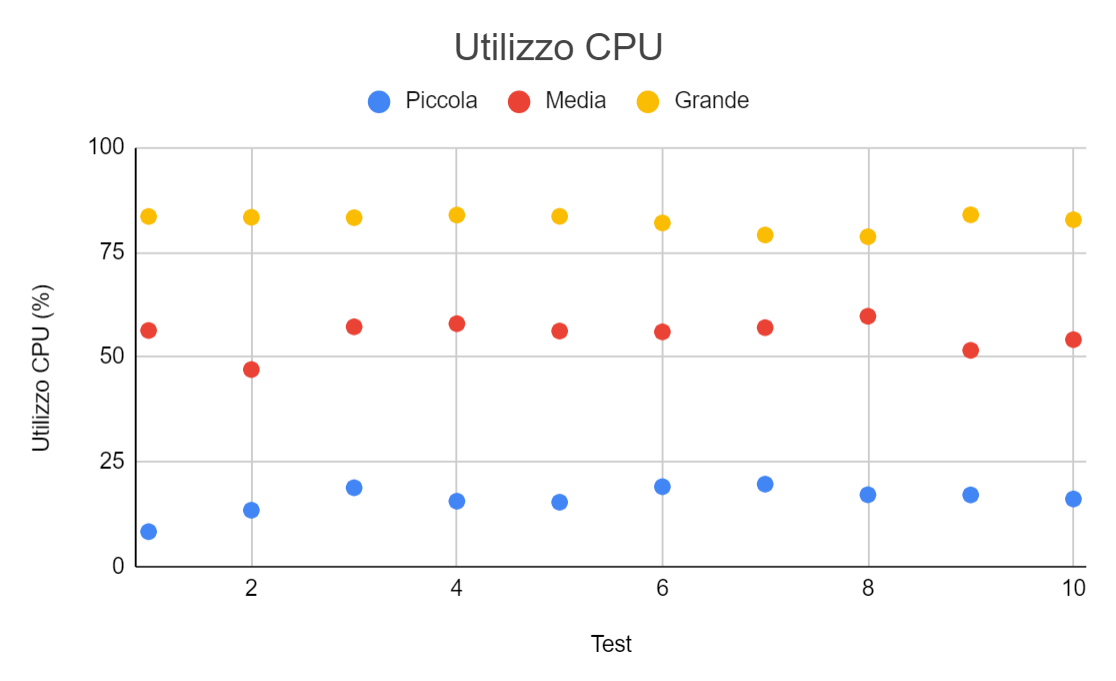
\includegraphics[width=1\columnwidth]{images/rust_cpu.png}
    \end{center}
    \caption{Utilizzo CPU misurato utilizzando Rust in combinazione con WebAssembly.}
\end{figure}
\begin{figure}
    \begin{center}
            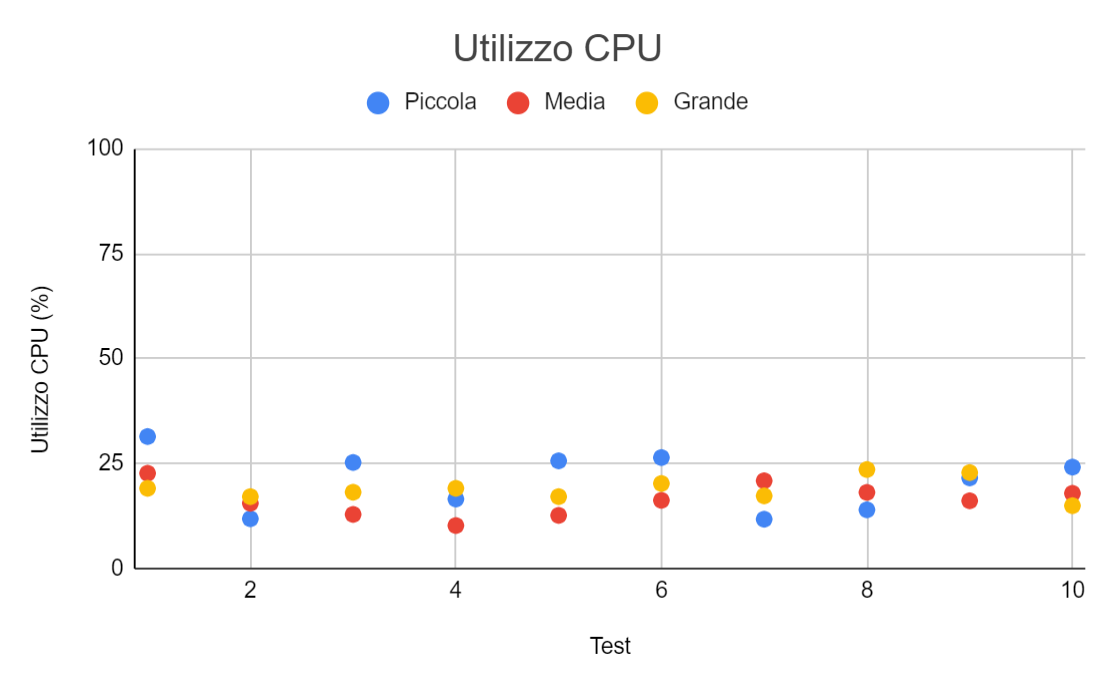
\includegraphics[width=1\columnwidth]{images/node_cpu.png}
    \end{center}
    \caption{Utilizzo CPU misurato utilizzando Node.js}
\end{figure}
\newpage
\subsection{Consumo memoria}
Come menzionato in precedenza, l'ultimo test eseguito riguarda il consumo di memoria durante l'esecuzione di una richiesta di elaborazione. 
\\Per quanto riguarda Rust sono stati ottenuti i seguenti risultati relativi al consumo di memoria:
\begin{align*}
    E[X]_{small}&=50.24\text{MB},  & \sigma_X=4.91\text{MB}\\
    E[X]_{medium}&=48.79.\text{MB},  & \sigma_X=1.02\text{MB}\\
    E[X]_{large}&=47.51.\text{MB},  & \sigma_X=0.90\text{MB}\\
\end{align*}
Per quanto riguarda Node.js, invece:
\begin{align*}
    E[X]_{small}&=80.51\text{MB},  & \sigma_X=2.73\text{MB}\\
    E[X]_{medium}&=79.80\text{MB},  & \sigma_X=1.16\text{MB}\\
    E[X]_{large}&=79.92\text{MB},  & \sigma_X=1.55\text{MB}\\
\end{align*}
Durante quest'ultima analisi, i risultati ottenuti sono stati molto simili per entrambi gli approcci, ma sostanzialmente differenti rispetto ai test precedenti.
\\In particolare, Node.js presenta un consumo di memoria leggermnete maggiore, ma in entrambi i casi, tale parametro viene mantenuto pressochè costante per ciascuna tipologia di immagine, non presentando differenze significative.
\newpage
\begin{figure}
    \begin{center}
            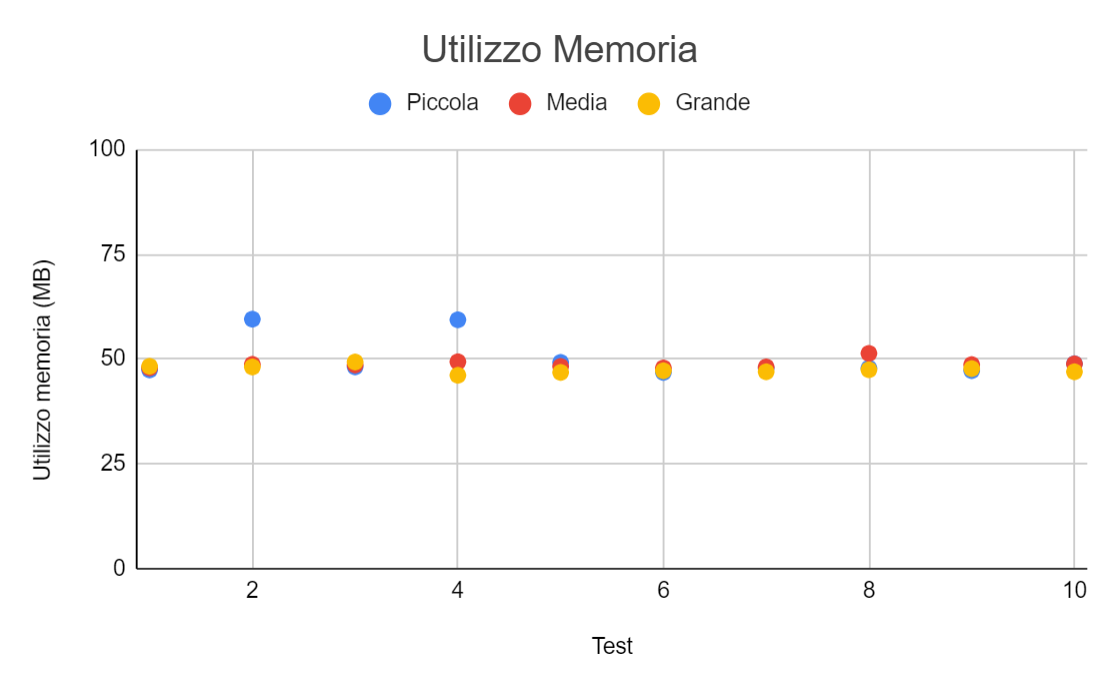
\includegraphics[width=1\columnwidth]{images/rust_mem.png}
    \end{center}
    \caption{Consumo di memoria misurato utilizzando Rust in combinazione con Wasm.}
\end{figure}
\begin{figure}
    \begin{center}
            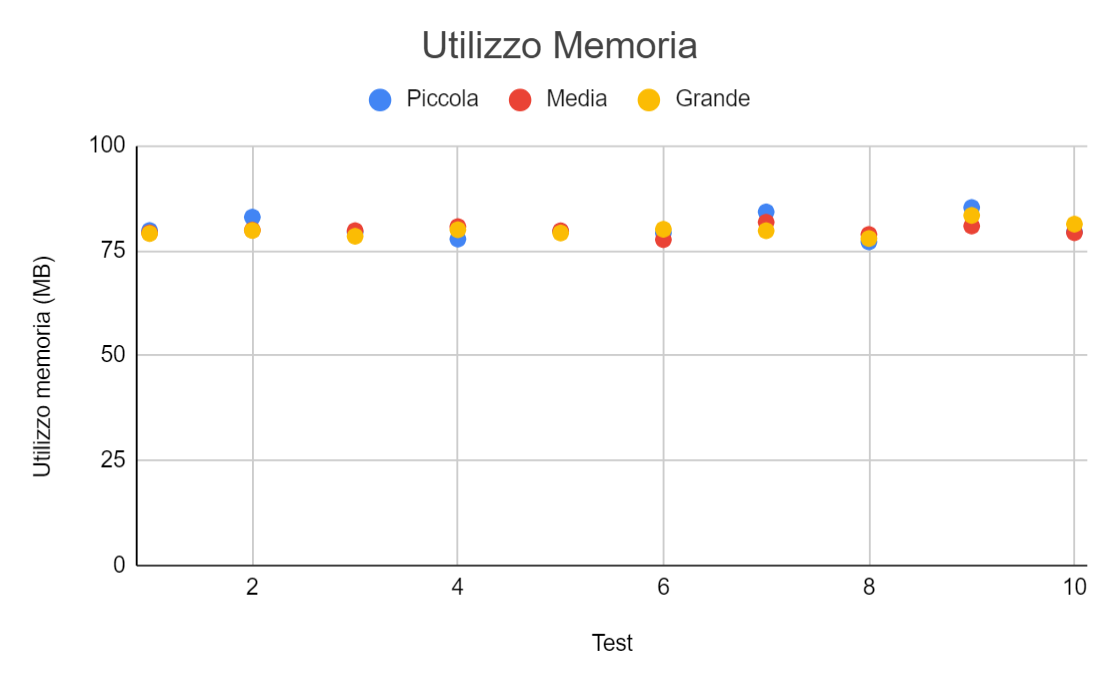
\includegraphics[width=1\columnwidth]{images/node_mem.png}
    \end{center}
    \caption{Consumo di memoria misurato utilizzando Node.js}
\end{figure}
\section{Conclusioni}
Per concludere questo lavoro di tesi, vengono presentate le considerazioni derivate dai risultati precedentemente esposti.
\\In primo luogo, è emerso che l'approccio basato su Rust e WebAssembly rappresenta una scelta eccellente in situazioni caratterizzate da operazioni ad alta intensità computazionale. Tuttavia, si rende necessaria un'analisi approfondita per determinare le funzionalità dell'applicazione che potrebbero effettivamente beneficiare di un'implementazione attraverso WebAssembly.
\\L'integrazione di codice Wasm all'interno di un programma Rust si è rivelata tutt'altro che immediata, comportando inoltre un overhead non trascurabile per un'applicazione che deve gestire un elevato volume di richieste.
\\D'altro canto Node.js offre un approccio di sviluppo più lineare e accessibile, specialmente per coloro che provengono dalle tecnologie web e posseggono una conoscenza consolidata del linguaggio JavaScript.
\\Tuttavia, l'adozione di Node.js potrebbe introdurre ulteriori sfide in quanto, per sua natura, risulta più indicato per applicazioni che fanno un ampio utilizzo del file system.
\\Durante lo svolgimento dei test è stato possibile notare, che Node.js introduce tempi di latenza peggiori rispetto a Wasm già con immagini relativamente piccole per gli standard odierni (5 Megapixel, 4,6 MegaByte). Inoltre è stata evidenziata una scarsa capacità nello sfruttare appieno la CPU, con un utilizzo che è rimasto praticamente costante durante tutti i test.
\\In conclusione è possibile affermare che l'utilizzo di WebAssembly server side possa rappresentare una scelta ottimale per applicazioni che devono gestire richieste comportanti un elevato numero di calcoli da parte della CPU.
Tuttavia, è importante evitare un uso eccessivo di questa tecnologia per richieste troppo semplici, al fine di prevenire un overhead non necessario e che potrebbe essere evitato anche utilizzando un linguaggio interpretato come JavaScript. 

%\appendix
% INCLUSIONE APPENDICI - - PERSONALIZZARE - TENERE COERENTE CON LISTA IN ALTO
%\chapter{An appendix}
\label{app:a}
% DA RIMUOVERE - LOREM IPSUM PER DIMOSTRAZIONE
\foreignlanguage{english}{\Blindtext}


%%%%%%%%%%%%%%%%%%%%%%%%%%%%%%%%%%%%%%%%%%%%%%%%%%%%%%%%%%%%%%%

% RINGRAZIAMENTI - PERSONALIZZARE
%\ringraziamenti
%Grazie a Grazia, Graziella e la sorella.

%%%%%%%%%%%%%%%%%%%%%%%%%%%%%%%%%%%%%%%%%%%%%%%%%%%%%%%%%%%%%%%

% BIBLIOGRAFIA
\phantomsection
\addcontentsline{toc}{chapter}{\refname}
\nocite{*}
\printbibliography

\end{document}
